% ==== Document Class & Packages =====
\documentclass[12pt,hidelinks]{article}
	\usepackage[explicit]{titlesec}
	\usepackage{titletoc}
	\usepackage{tocloft}
	\usepackage{charter}
	\usepackage[many]{tcolorbox}
	\usepackage{amsmath}
	\usepackage{graphicx}
	\usepackage{xcolor}
	\usepackage{tikz,lipsum,lmodern}
	\usetikzlibrary{calc}
	\usepackage[english]{babel}
	\usepackage[utf8]{inputenc}
	\usepackage{fancyhdr}
	\usepackage{mathrsfs}
	\usepackage{empheq}
	\usepackage{fourier}% change to lmodern if fourier is no available
	\usepackage{wrapfig}
	\usepackage{fancyref}
	\usepackage{hyperref}
	\usepackage{cleveref}
	\usepackage{listings}
	\usepackage{varwidth}
	\usepackage{longfbox}
	\usepackage{geometry}
	\usepackage{marginnote}
	\usepackage{setspace}
	%\usepackage{subfigure}
	\usepackage{minted}
	\tcbuselibrary{theorems}
	\tcbuselibrary{breakable, skins}
	\tcbuselibrary{listings, documentation}
	\geometry{
		a4paper,
		left=33mm,
		right=33mm,
		top=20mm}
% ========= Path to images ============
%   - Direct the computer on the path 
% 	  to the folder containg the images
% =====================================
\graphicspath{{./images/}}
% ============= Macros ================
\newcommand{\fillin}{\underline{\hspace{.75in}}{\;}}
\newcommand{\solution}{\textcolor{mordantred19}{Solution:}}
\setlength{\parindent}{0pt}
\addto{\captionsenglish}{\renewcommand*{\contentsname}{Table of Contents}}
\linespread{1.2}
% ======== Footers & Headers ==========
\cfoot{\thepage}
\chead{}\rhead{}\lhead{}
% =====================================
\renewcommand{\thesection}{\arabic{section}}
\newcommand\sectionnumfont{% font specification for the number
	\fontsize{380}{130}\color{myblueii}\selectfont}
\newcommand\sectionnamefont{% font specification for the name "PART"
	\normalfont\color{white}\scshape\small\bfseries }
% ============= Colors ================
% ----- Red -----
\definecolor{mordantred19}{rgb}{0.68, 0.05, 0.0}
% ----- Blue -----
\definecolor{st.patrick\'sblue}{rgb}{0.14, 0.16, 0.48}
\definecolor{teal}{rgb}{0.0, 0.5, 0.5}
\definecolor{beaublue}{rgb}{0.74, 0.83, 0.9}
\definecolor{mybluei}{RGB}{0,173,239}
\definecolor{myblueii}{RGB}{63,200,244}
\definecolor{myblueiii}{RGB}{199,234,253}
% ---- Yellow ----
\definecolor{blond}{rgb}{0.98, 0.94, 0.75}
\definecolor{cream}{rgb}{1.0, 0.99, 0.82}
% ----- Green ------
\definecolor{emerald}{rgb}{0.31, 0.78, 0.47}
\definecolor{darkspringgreen}{rgb}{0.09, 0.45, 0.27}
% ---- White -----
\definecolor{ghostwhite}{rgb}{0.97, 0.97, 1.0}
\definecolor{splashedwhite}{rgb}{1.0, 0.99, 1.0}
% ---- Grey -----
\definecolor{whitesmoke}{rgb}{0.96, 0.96, 0.96}
\definecolor{lightgray}{rgb}{0.92, 0.92, 0.92}
\definecolor{floralwhite}{rgb}{1.0, 0.98, 0.94}
% ========= Part Format ==========
\titleformat{\section}
{\normalfont\huge\filleft}
{}
{20pt}
{\begin{tikzpicture}[remember picture,overlay]
	\fill[myblueiii] 
	(current page.north west) rectangle ([yshift=-13cm]current page.north east);   
\node[
	fill=mybluei,
	text width=2\paperwidth,
	rounded corners=6cm,
	text depth=18cm,
	anchor=center,
	inner sep=0pt] at (current page.north east) (parttop)
	{\thepart};%
\node[
	anchor=south east,
	inner sep=0pt,
	outer sep=0pt] (partnum) at ([xshift=-20pt]parttop.south) 
	{\sectionnumfont\thesection};
\node[
	anchor=south,
	inner sep=0pt] (partname) at ([yshift=2pt]partnum.south)   
	{\sectionnamefont SECTION};
\node[
	anchor=north east,
	align=right,
	inner xsep=0pt] at ([yshift=-0.5cm]partname.east|-partnum.south) 
	{\parbox{.7\textwidth}{\raggedleft#1}};
\end{tikzpicture}%
}
% ========= Hyper Ref ===========
\hypersetup{
	colorlinks,
	linkcolor={red!50!black},
	citecolor={blue!50!black},
	urlcolor={blue!80!black}
}
% ========= Example Boxes =============
\tcbset{
	defstyle/.style={
		fonttitle=\bfseries\upshape, 
		fontupper=\slshape,
		arc=0mm, 
		beamer,
		colback=blue!5!white,
		colframe=blue!75!black},
	theostyle/.style={
		fonttitle=\bfseries\upshape, 
		fontupper=\slshape,
		colback=red!10!white,
		colframe=red!75!black},
	visualstyle/.style={
		height=6.5cm,
		breakable,
		enhanced,
		leftrule=0pt,
		rightrule=0pt,
		bottomrule=0pt,
		outer arc=0pt,
		arc=0pt,
		colframe=mordantred19,
		colback=lightgray,
		attach boxed title to top left,
		boxed title style={
			colback=mordantred19,
			outer arc=0pt,
			arc=0pt,
			top=3pt,
			bottom=3pt,
		},
		fonttitle=\sffamily,},
	discussionstyle/.style={
		height=6.5cm,
		breakable,
		enhanced,
		rightrule=0pt,
		toprule=0pt,
		outer arc=0pt,
		arc=0pt,
		colframe=mordantred19,
		colback=lightgray,
		attach boxed title to top left,
		boxed title style={
			colback=mordantred19,
			outer arc=0pt,
			arc=0pt,
			top=3pt,
			bottom=3pt,
		},
		fonttitle=\sffamily},
	mystyle/.style={
		height=6.5cm,
		breakable,
		enhanced,
		rightrule=0pt,
		leftrule=0pt,
		bottomrule=0pt,
		outer arc=0pt,
		arc=0pt,
		colframe=mordantred19,
		colback=lightgray,
		attach boxed title to top left,
		boxed title style={
			colback=mordantred19,
			outer arc=0pt,
			arc=0pt,
			top=3pt,
			bottom=3pt,
		},
		fonttitle=\sffamily},
	aastyle/.style={
			height=3.5cm,
			enhanced,
			colframe=teal,
			colback=lightgray,
			colbacktitle=floralwhite,
			fonttitle=\bfseries,
			coltitle=black,
		attach boxed title to top center={
	  		yshift=-0.25mm-\tcboxedtitleheight/2,
	   		yshifttext=2mm-\tcboxedtitleheight/2}, 
		boxed title style={boxrule=0.5mm,
			frame code={ \path[tcb fill frame] ([xshift=-4mm]frame.west)
				-- (frame.north west) -- (frame.north east) -- ([xshift=4mm]frame.east)
				-- (frame.south east) -- (frame.south west) -- cycle; },
			interior code={ 
				\path[tcb fill interior] ([xshift=-2mm]interior.west)
				-- (interior.north west) -- (interior.north east)
				-- ([xshift=2mm]interior.east) -- (interior.south east) -- (interior.south west)
				-- cycle;} }
				},
	examstyle/.style={
		height=9.5cm,
		breakable,
		enhanced,
		rightrule=0pt,
		leftrule=0pt,
		bottomrule=0pt,
		outer arc=0pt,
		arc=0pt,
		colframe=mordantred19,
		colback=lightgray,
		attach boxed title to top left,
		boxed title style={
			colback=mordantred19,
			outer arc=0pt,
			arc=0pt,
			top=3pt,
			bottom=3pt,
		},
		fonttitle=\sffamily},
	doc head command={
		interior style={
			fill,
			left color=yellow!20!white, 
			right color=white}},
	doc head environment={
		boxsep=4pt,
		arc=2pt,
		colback=yellow!30!white,
		},
	doclang/environment content=text
}
% ============= Boxes ================
\newtcolorbox[auto counter,number within=section]{example}[1][]{
	mystyle,
	title=Example~\thetcbcounter,
	overlay unbroken and first={
		\path
		let
		\p1=(title.north east),
		\p2=(frame.north east)
		in
		node[anchor=
			west,
			font=\sffamily,
			color=st.patrick\'sblue,
			text width=\x2-\x1] 
		at (title.east) {#1};
	}
}
\newtcolorbox[auto counter,number within=section]{longexample}[1][]{
	examstyle,
	title=Example~\thetcbcounter,
	overlay unbroken and first={
		\path
		let
		\p1=(title.north east),
		\p2=(frame.north east)
		in
		node[anchor=
		west,
		font=\sffamily,
		color=st.patrick\'sblue,
		text width=\x2-\x1] 
		at (title.east) {#1};
	}
}
\newtcolorbox[auto counter,number within=section]{example2}[1][]{
	aastyle,
	title=Example~\thetcbcounter,{}
}
\newtcolorbox[auto counter,number within=section]{discussion}[1][]{
	discussionstyle,
	title=Discussion~\thetcbcounter,
	overlay unbroken and first={
		\path
		let
		\p1=(title.north east),
		\p2=(frame.north east)
		in
		node[anchor=
		west,
		font=\sffamily,
		color=st.patrick\'sblue,
		text width=\x2-\x1] 
		at (title.east) {#1};
	}
}
\newtcolorbox[auto counter,number within=section]{visualization}[1][]{
	visualstyle,
	title=Visualization~\thetcbcounter,
	overlay unbroken and first={
		\path
		let
		\p1=(title.north east),
		\p2=(frame.north east)
		in
		node[anchor=
		west,
		font=\sffamily,
		color=st.patrick\'sblue,
		text width=\x2-\x1] 
		at (title.east) {#1};
	}
}
% --------- Theorems ---------
\newtcbtheorem[number within=subsection,crefname={definition}{definitions}]%
	{Definition}{Definition}{defstyle}{def}%
\newtcbtheorem[use counter from=Definition,crefname={theorem}{theorems}]%
	{Theorem}{Theorem}{theostyle}{theo}
	%
\newtcbtheorem[use counter from=Definition]{theo}{Theorem}%
{
	theorem style=plain,
	enhanced,
	colframe=blue!50!black,
	colback=yellow!20!white,
	coltitle=red!50!black,
	fonttitle=\upshape\bfseries,
	fontupper=\itshape,
	drop fuzzy shadow=blue!50!black!50!white,
	boxrule=0.4pt}{theo}
\newtcbtheorem[use counter from=Definition]{DashedDefinition}{Definition}%
 {
 	enhanced,
 	frame empty,
 	interior empty,
 	colframe=darkspringgreen!50!white,
	coltitle=darkspringgreen!50!black,
	fonttitle=\bfseries,
	colbacktitle=darkspringgreen!15!white,
	borderline={0.5mm}{0mm}{darkspringgreen!15!white},
	borderline={0.5mm}{0mm}{darkspringgreen!50!white,dashed},
	attach boxed title to top center={yshift=-2mm},
	boxed title style={boxrule=0.4pt},
	varwidth boxed title}{theo}
%%%%%%%%%%%%%%%%%%%%%%%%%%%%%%%%%%%%%%%%
\newtcblisting[auto counter,number within=section]{disexam}{
	skin=bicolor,
	colback=white!30!beaublue,
	colbacklower=white,
	colframe=black,
	before skip=\medskipamount,
	after skip=\medskipamount,
	fontlower=\footnotesize,
	listing options={style=tcblatex,texcsstyle=*\color{red!70!black}},}
%%%%%%%%%%%%%%%%%%%%%%%%%%%%%%%%%%%%%%%

\begin{document}
\begin{titlepage}
	\centering % Center everything on the title page
	\scshape % Use small caps for all text on the title page
	\vspace*{1.5\baselineskip} % White space at the top of the page
% ===================
%	Title Section 	
% ===================

	\rule{13cm}{1.6pt}\vspace*{-\baselineskip}\vspace*{2pt} % Thick horizontal rule
	\rule{13cm}{0.4pt} % Thin horizontal rule
	
		\vspace{0.75\baselineskip} % Whitespace above the title
% ========== Title ===============	
	{	\Huge Dspace\\ 
			\vspace{4mm}
		MANUAL  \\	}
% ======================================
		\vspace{0.75\baselineskip} % Whitespace below the title
	\rule{13cm}{0.4pt}\vspace*{-\baselineskip}\vspace{3.2pt} % Thin horizontal rule
	\rule{13cm}{1.6pt} % Thick horizontal rule
	
		\vspace{1.75\baselineskip} % Whitespace after the title block
% =================
%	Information	
% =================
	{\large Leonard \\
		\vspace*{1.2\baselineskip}
	EMAIL: leonardcampelo@ibict.br} \\
	\vfill

\end{titlepage}
%%%%%%%%%%%%%%%%%%%%%%%%%%%%%%%%%%%%%%%%%%%%%%%%%%%%%%%%%%%
\tableofcontents
\vfill
\small{\noindent \textbf{About This File} \vspace{-3mm}\\
\noindent \rule{3.3cm}{0.5pt} \\
This file was created for the benefit of all teachers and students wanting to use Latex for tests/exams/lessons/thesis/articles etc.\\
The entirety of the contents within this file, and folder, are free for public use.}
\newpage
\newgeometry{
	left=29mm, 
	right=29mm, 
	top=20mm, 
	bottom=15mm}
%%%%%%%%%%%%%%%%%%%%%%%%%%%%%%%%%%%%%%%%%%%%%%%%%%%%%%%%%%%
\section{Introdução}
\newpage
    \subsection{O que é o DSpace?}
        Este manual oferece instruções sobre o uso do software DSpace. Além da instalação e configurações básicas.
        O DSpace é um dos softwares mais utilizados mundialmente para construção e gerenciamento de repositórios digitais e que apesar de ser uma ferramenta simples dispõe de muitos recursos.
        \singlespacing
        A utilização crescente do software para repositórios pelas instituições brasileiras e as constantes atualizações e mudanças ocorridas foram fatores que impulsionaram a criação deste manual. 
         \singlespacing
         Utilizando a versão 6.3 do DSpace, este documento foi estruturado contendo as principais funcionalidades necessárias para a gestão de um repositório digital, focando principalmente repositórios institucionais. Esclarece ainda sobre temas correlatos que podem auxiliar os gestores na qualidade de dados de seus repositórios como: as diretrizes de metadados e a ferramenta para correção de dado, OpenRefine.
        \singlespacing
        O manual está composto por seções explicando o funcionamento do DSpace, a estrutura em que as informações são organizadas, as principais ferramentas disponíveis para os administradores dos repositórios, como realizar o depósito de um documento, as tarefas que envolvem o fluxo de depósito, breves explicações sobre o formulário de entrada, informações sobre as principais diretrizes de metadados e esclarecimentos sobre o uso da ferramenta Google OpenRefine.
\newpage
        \singlespacing
\section{Como funciona o DSpace}
\newpage
    \subsection{Visão geral:}
        \singlespacing \textbullet \hspace{6pt} Crie as estruturas de armazenamento: comunidades, subcomunidades e coleções;
        
        \textbullet \hspace{6pt} Defina as políticas das comunidades, subcomunidades e coleções: como será o fluxo de depósito; quem poderá depositar em cada coleção; configurações de acesso – aberto, restrito ou embargado.

        \textbullet \hspace{6pt} Atribua permissões aos usuários do repositório: defina quem poderá fazer depósitos; quem poderá editar e excluir depósitos; quem fará a avaliação e revisão dos depósitos; quais serão os administradores;

        \subsection{Sobre as permissões}
        O gerenciamento do DSpace é realizado por meio de diferentes permissões de acesso. Isso significa que os usuários cadastrados no sistema podem ter funções diferentes e, por isso, têm acesso a diferentes funcionalidades e ferramentas do sistema. O usuário administrador é o único que pode realizar todas as ações no sistema, pode também delegar funções e permissões para outros usuários, inclusive dar permissões de administrador para outros usuários.
        
        \subsection{Sobre as políticas}
        É possível criar políticas para cada elemento integrante do repositório:
        
            \centerline{Comunidade}      
            \centerline{Subcomunidade}      
            \centerline{Coleção}      
            \centerline{Item}      
            \centerline{Bitstream}
        \singlespacing
        A política aplicada ao item será sempre aquela atribuída ao elemento de menor hierarquia. Por exemplo, uma determinada coleção possui uma política de tornar todos os seus itens disponíveis ao público geral (permissão READ ao grupo Anonymous). Contudo, um item pertencente a esta coleção pode ter uma política que restrinja o acesso a ele, mesmo que a coleção da qual faz parte (hierarquia superior) tenha uma política diferente. Da mesma forma, o item pode ser composto de vários arquivos (bitstreams) e restringir o acesso a apenas um ou alguns desses arquivos, já que é possível atribuir políticas específicas ao bitstream.
        \singlespacing
        \textbf{\underline{NOTA}}: \emph{Bitstreams}  são os arquivos de computadores comuns. Por exemplo, o arquivo PDF de uma tese é um \emph{bitstream} no contexto dos repositórios.
        \singlespacing
        \textbf{\underline{IMPORTANTE}}: se você alterar a política de uma coleção que já possui itens, a nova política só valerá para os itens depositados depois da mudança. Os itens existentes permanecerão com as políticas antigas, ou seja, não serão atualizados automaticamente. Para atualizá-los, siga os procedimentos descritos em 5.3.4 Ferramenta avançada de administração de políticas.
\newpage
        Visualização das comunidades e coleções:
        
        \begin{figure}[!htp]
                \centering
                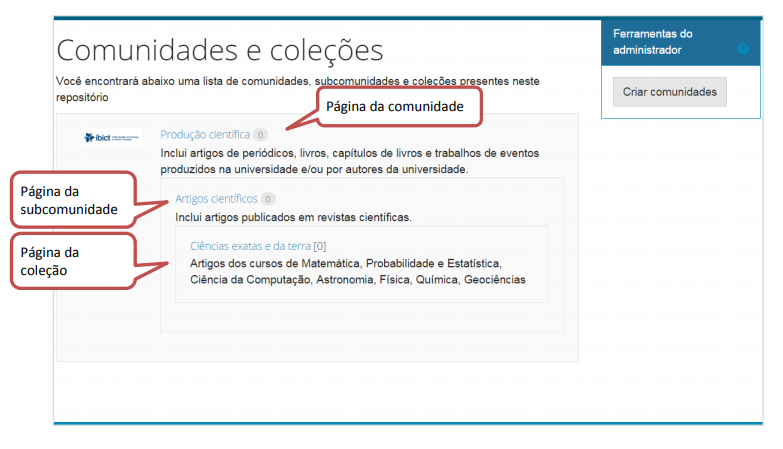
\includegraphics[scale=0.8]{figura/Figura1.png}
                \caption{Visualização das comunidades e coleções}
            \label{Rotulo}
        \end{figure}
        
\newpage
\section{Logar no repositório}
\newpage
    Para fazer o login no sistema é necessário ser um usuário registrado e ter uma senha de acesso. Para se registrar no sistema, siga os passos abaixo (1-6). Caso você já seja cadastrado no sistema pule para o passo 7
    \subsection{Registrar novo usuário no repositório}
    
    Passo 1: Na barra superior, clique no menu “Entrar em:” e acesse <Meu espaço>.
     \begin{figure}[!htp]
                \centering
                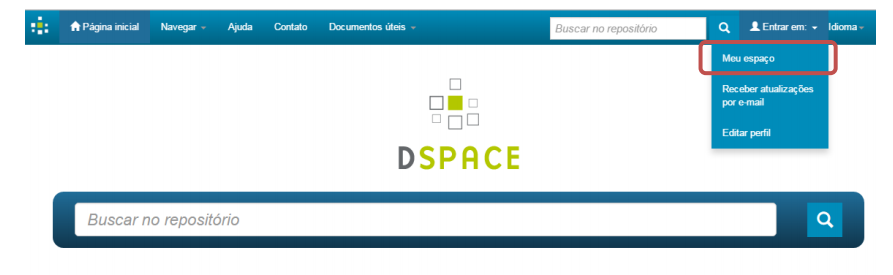
\includegraphics[scale=0.7]{figura/Figura2.png}
                \caption{Meu espaço}
            \label{Rotulo}
        \end{figure}   
        
       Passo 2 : Clique em <Usuário novo? Clique aqui para se registrar>. 
       
       \begin{figure}[!htp]
                \centering
                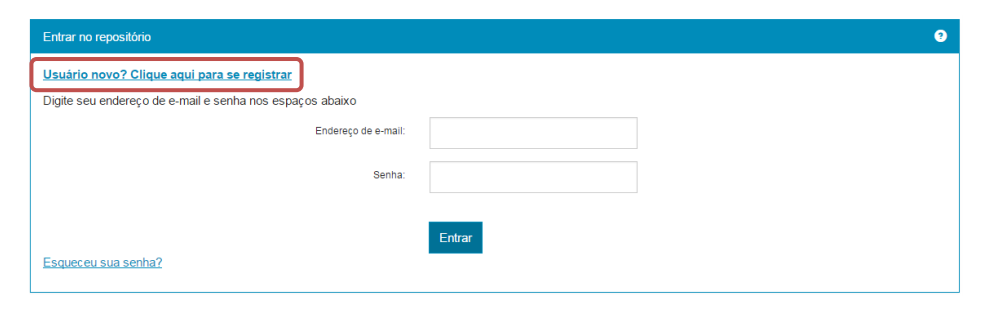
\includegraphics[scale=0.6]{figura/Figura3.png}
                \caption{Figura 3 - Cadastro de novo usuário}
            \label{Rotulo}
        \end{figure}  
        
    
        Passo 3: Informe seu endereço de e-mail que será cadastrado no sistema e clique em <Registrar>. Note que o endereço de e-mail cadastrado será utilizado para o envio de mensagens do sistema para você.
        
        \begin{figure}[!htp]
                \centering
                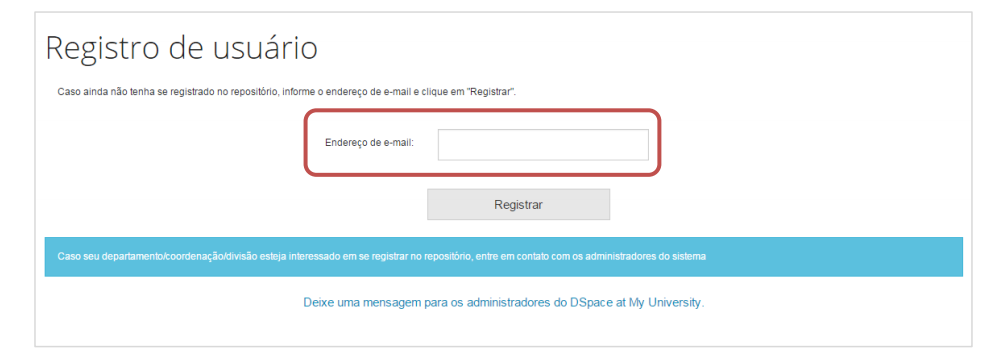
\includegraphics[scale=0.6]{figura/Figura4.png}
                \caption{Registro de usuário}
            \label{Rotulo}
        \end{figure}
\newpage        
        Passo 4: Após informar o endereço de e-mail e clicar em registrar, deverá aparecer uma mensagem informando que seu e-mail foi registrado e que você receberá uma mensagem no e-mail cadastrado. Caso isto não aconteça repita o passo três.
        
        \begin{figure}[!htp]
                \centering
                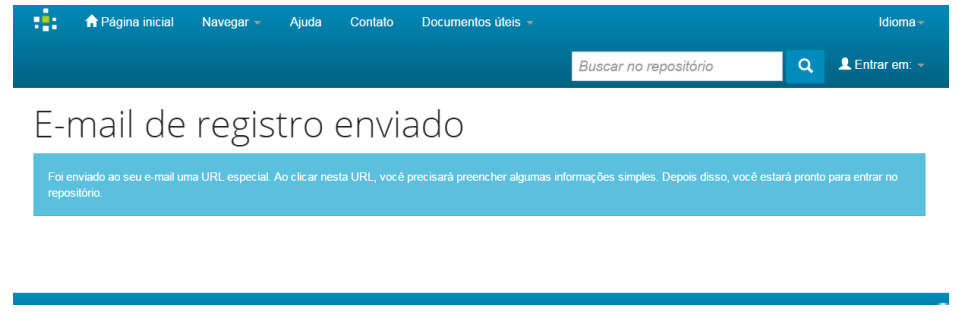
\includegraphics[scale=0.6]{figura/Figura5.png}
                \caption{Confirmação de registro}
            \label{Rotulo}
        \end{figure}
        
        Passo 5: Abra a mensagem que você recebeu na conta de e-mail registrada e clique no link que foi enviado.
        \singlespacing
        Passo 6: Ao clicar no link, uma nova página do repositório será aberta. Preencha as informações solicitadas e clique em <Complete o registro>. É obrigatório o preenchimento do “Primeiro nome” e do “Último nome”. 
        
        \begin{figure}[!htp]
                \centering
                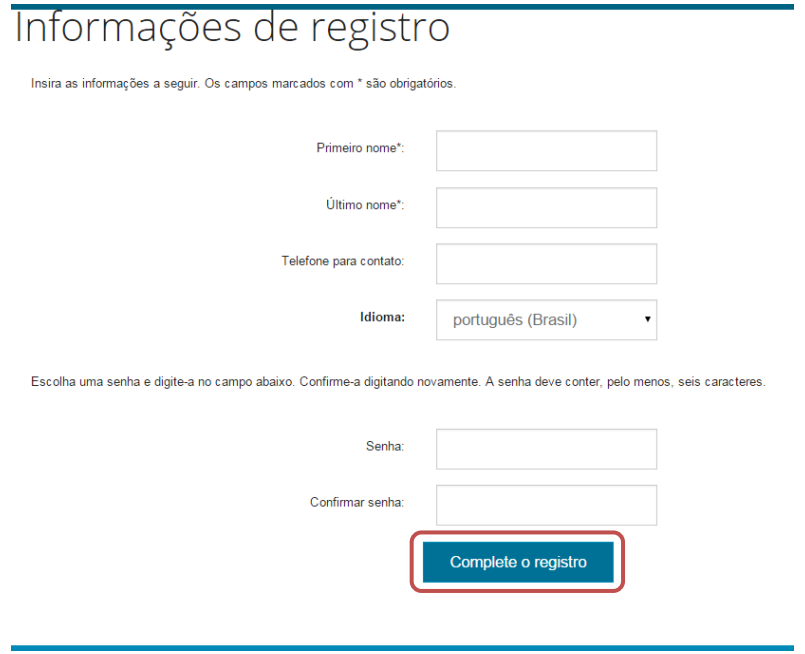
\includegraphics[scale=0.5]{figura/Figura6.png}
                \caption{Confirmação de registro}
            \label{Rotulo}
        \end{figure}
        
\newpage
        \subsection{Logar no repositório a partir de uma conta já existente}
        
        Passo 7: Na barra superior, clique no menu “Entrar em:” e acesse <Meu espaço>.
        
        \begin{figure}[!htp]
                \centering
                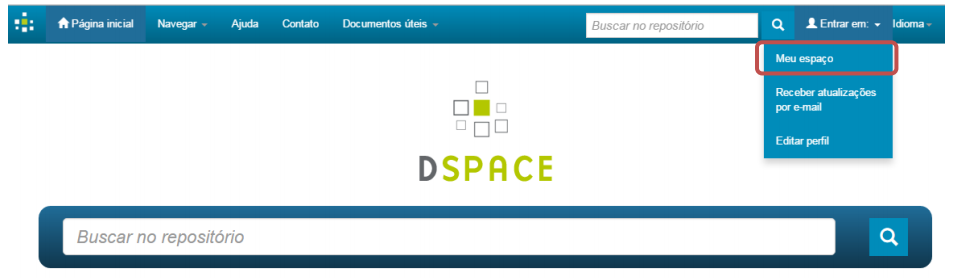
\includegraphics[scale=0.6]{figura/Figura7.png}
                \caption{Meu espaço}
            \label{Rotulo}
        \end{figure}
        
        Passo 8: Informe o endereço de e-mail cadastrado no repositório, a senha de acesso e clique em <Entrar>.
        
        \begin{figure}[!htp]
                \centering
                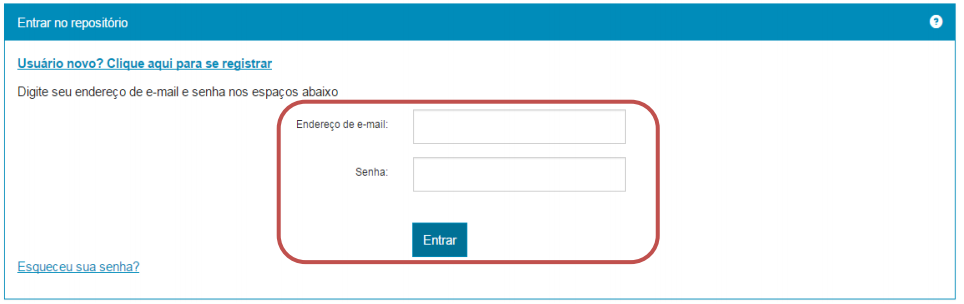
\includegraphics[scale=0.6]{figura/Figura8.png}
                \caption{Entrar no repositório}
            \label{Rotulo}
        \end{figure}
        
\newpage
        Passo 9: Acesso à “Meu espaço”. Após o login, você será direcionado a página <Meu espaço>, que apresenta as opções de iniciar um novo depósito, visualizar depósitos aceitos ou ver as tarefas pendentes:
        
        \begin{figure}[!htp]
                \centering
                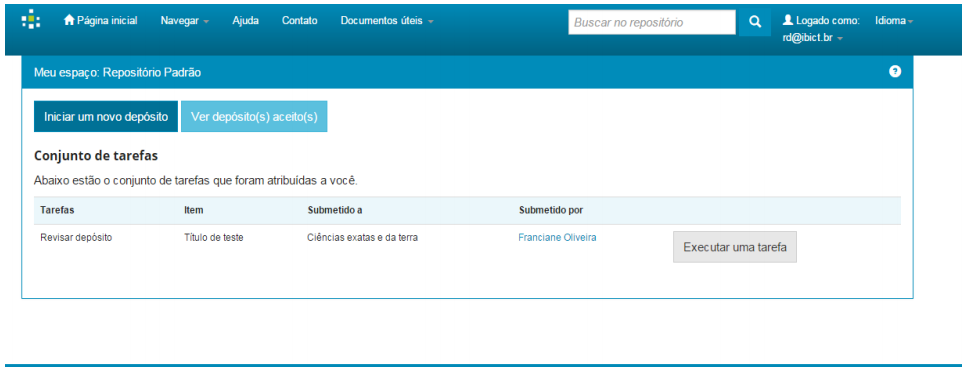
\includegraphics[scale=0.6]{figura/Figura9.png}
                \caption{Acesso à página “Meu espaço”}
            \label{Rotulo}
        \end{figure}
        
        
\newpage        
\section{Criar comunidades, subcomunidades e coleções}
\newpage

    Para iniciar o depósito de arquivos no repositório é recomendável que sejam criadas as
    estruturas de \underline{comunidades}, \underline{subcomunidades} e \underline{coleções}. 
    \singlespacing
    A criação destas três estruturas não é obrigatória. É possível criar uma única comunidade e depositar todos os arquivos na mesma comunidade. No entanto, a estrutura de comunidades, subcomunidades e coleções possui a funcionalidade de organizar o conteúdo dentro do repositório, permitindo assim melhor navegabilidade e atribuição de políticas e permissões diferenciadas segundo necessidades determinadas. Um exemplo de organização em comunidades, subcomunidades e coleções é apresentado a seguir:
    
    \begin{figure}[!htp]
                \centering
                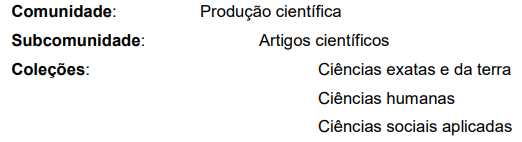
\includegraphics[scale=0.6]{figura/Comunidades.png}
            \label{Rotulo}
        \end{figure}
    
        \subsection{Criação de comunidade}
        
        Passo 1: Na barra superior, clique no menu “Navegar” e acesse <Comunidades e coleções>. 
        
        \begin{figure}[!htp]
                \centering
                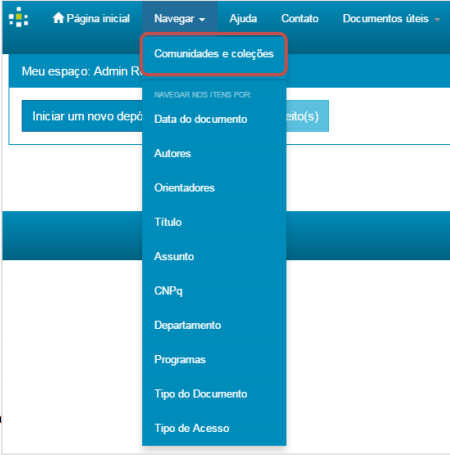
\includegraphics[scale=0.8]{figura/Figura10.png}
                \caption{Comunidades e coleções}
            \label{Rotulo}
        \end{figure}
    
\newpage
     Passo 2: Em ferramenta do administrador, clique em "Criar comunidades". 
     
     \begin{figure}[!htp]
                \centering
                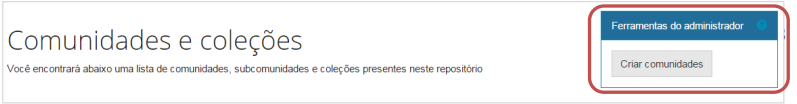
\includegraphics[scale=0.8]{figura/Figura11.png}
                \caption{Como criar comunidades}
            \label{Rotulo}
        \end{figure}
        
    Passo 3: Descreva a comunidade que será criada nos campos adequados e clique em <Criar>. Note que apenas o campo “Nome” é obrigatório, no entanto o preenchimento dos outros campos pode ser importante para prestar informações para os gestores que alimentarão a comunidade e para os usuários finais.
    
    \begin{figure}[!htp]
                \centering
                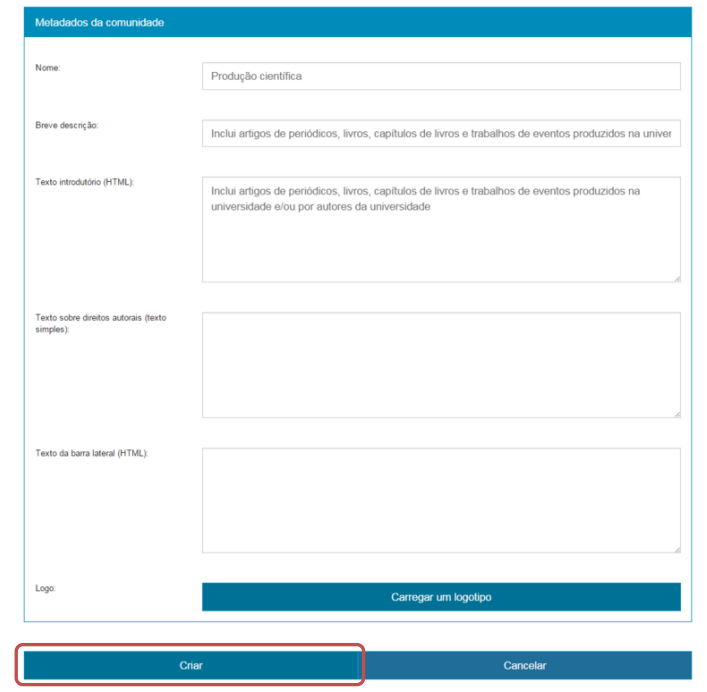
\includegraphics[scale=0.9]{figura/Figura12.png}
                \caption{Criar comunidade}
            \label{Rotulo}
        \end{figure}

\newpage
    Para saber mais sobre o preenchimento dos campos, siga as orientações abaixo:
    \singlespacing
    \textbullet \hspace{6pt} \textbf{Nome:} informe o nome que será dado à comunidade. Exemplo: Produção científica.
    \singlespacing
    \textbullet \hspace{6pt} \textbf{Texto introdutório (HTML):} insira um texto sobre a comunidade. Permite o uso de tags html que alteram a apresentação do texto. Exemplo: <p>Inclui artigos de periódicos, livros, capítulos de livros e trabalhos de eventos <b> produzidos na universidade </b> e/ou por autores da universidade.</p>
    \singlespacing
    \textbullet \hspace{6pt} \textbf{Texto sobre direitos autorais:} insira um texto sobre os direitos autorais que serão estabelecidos para os documentos da comunidade.
    \singlespacing
    \textbullet \hspace{6pt} \textbf{Texto da barra lateral:}  insira outro texto que queira para descrever a comunidade que aparecerá na barra lateral da página da comunidade.
    \singlespacing
    Passo 4: Atribuir um logotipo à comunidade. Ao criar uma comunidade é possível ainda relacioná-la ao seu logotipo, caso ela tenha uma imagem representativa. Para o uso do logo pela comunidade clique em <Carregar um logotipo>.
    
    \begin{figure}[!htp]
                \centering
                
\includegraphics[scale=0.8]{figura/Figura13.png}
                \caption{Carregar logotipo}
            \label{Rotulo}
        \end{figure}
        
    Passo 5: Clique em <Escolher arquivo> para selecionar uma imagem armazenada em seu computador. 
    
    \begin{figure}[!htp]
                \centering
                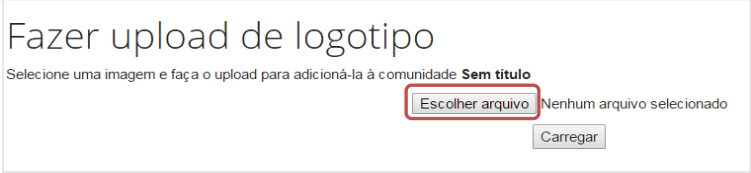
\includegraphics[scale=0.8]{figura/Figura14.png}
                \caption{Carregar logotipo}
            \label{Rotulo}
        \end{figure}
        
\newpage
    Passo 6: Selecione a imagem navegando pelas pastas de seu computador e clique em <Carregar>.
    
    \begin{figure}[!htp]
                \centering
                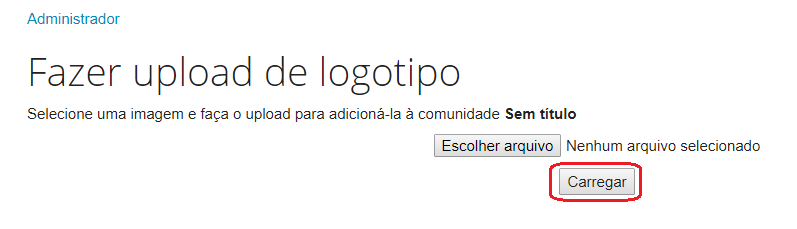
\includegraphics[scale=0.8]{figura/Figura15.png}
                \caption{Upload do arquivo}
            \label{Rotulo}
        \end{figure}
        
    Passo 7: Ao carregar o logotipo, a imagem poderá ser visualizada na página de gerenciamento da comunidade. Nela você poderá alterar a imagem carregada por outra, clicando em <Carregar novo logotipo> ou Excluir a imagem carregada, clicando em <Deletar (logotipo)>.
    
    \begin{figure}[!htp]
                \centering
                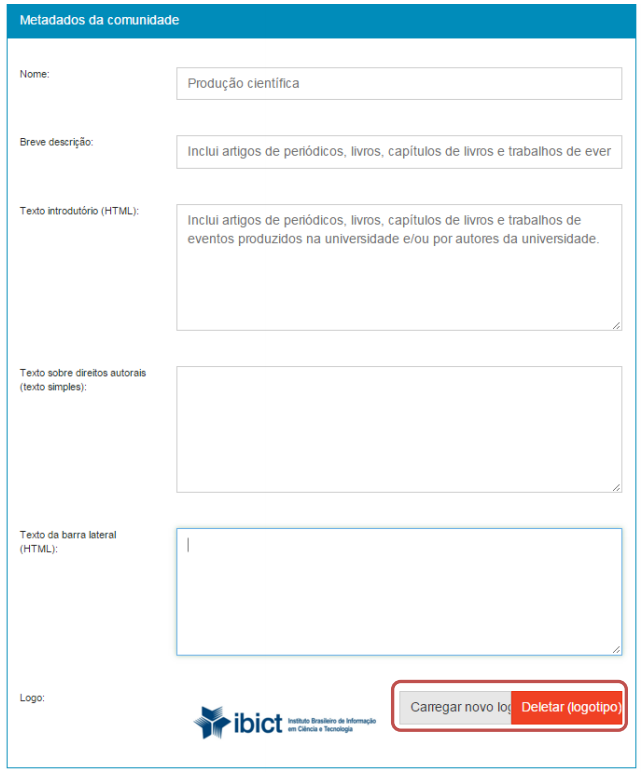
\includegraphics[scale=0.7]{figura/Figura16.png}
                \caption{Editar comunidade}
            \label{Rotulo}
        \end{figure}
        
    \subsection{Editar comunidade}
    
    Passo 1: Para editar alguma configuração da comunidade, entre na página da comunidade e clique em <Editar>.
    
    \begin{figure}[!htp]
                \centering
                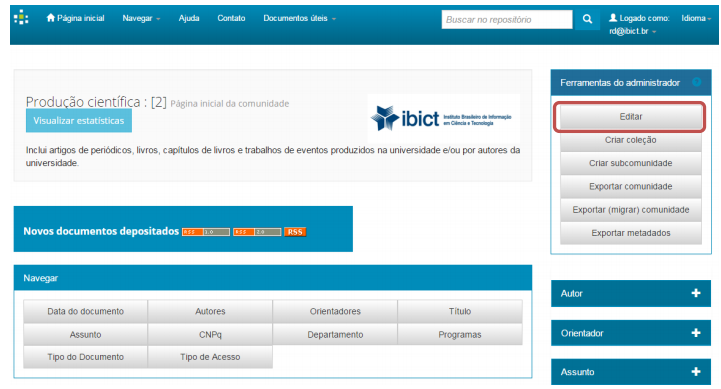
\includegraphics[scale=0.8]{figura/Figura17.png}
                \caption{Editar configuração da comunidade}
            \label{Rotulo}
        \end{figure}
        
    Passo 2: A página de edição assemelha-se com a imagem abaixo. Além de poder modificar a descrição da comunidade, você poderá:
    \singlespacing
    Excluir a comunidade, clicando em “Deletar esta comunidade”;
    Selecionar, mudar ou excluir os usuários administradores dessa comunidade;
    Estabelecer e editar políticas para a comunidade;
    Acessar as ferramentas de curadoria da comunidade.
    
    \begin{figure}[!htp]
                \centering
                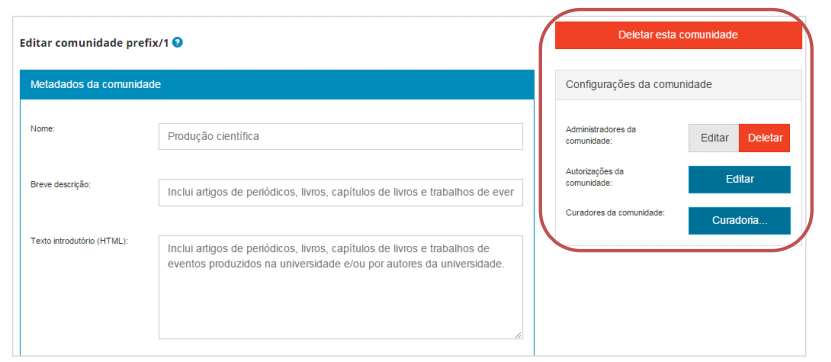
\includegraphics[scale=0.7]{figura/Figura18.png}
                \caption{Editar comunidade}
            \label{Rotulo}
        \end{figure}
        
\newpage
    \subsection{Estabelecimento de políticas para as comunidades}

    Para cada comunidade criada também é permitida a atribuição de grupos de usuários e políticas específicas para o seu gerenciamento.
    \singlespacing
    Passo 1: Acesse a página de edição da comunidade. Caminho:
    
    \begin{figure}[!htp]
                \centering
                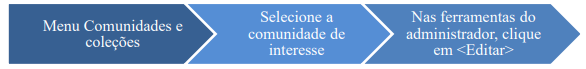
\includegraphics[scale=0.6]{figura/MenuComunidadesColecoes.png}
            \label{Rotulo}
        \end{figure}
    
    Passo 2: Clique em <Criar> para estabelecer um grupo de usuários como Administradores da comunidade.
    
    \begin{figure}[!htp]
                \centering
                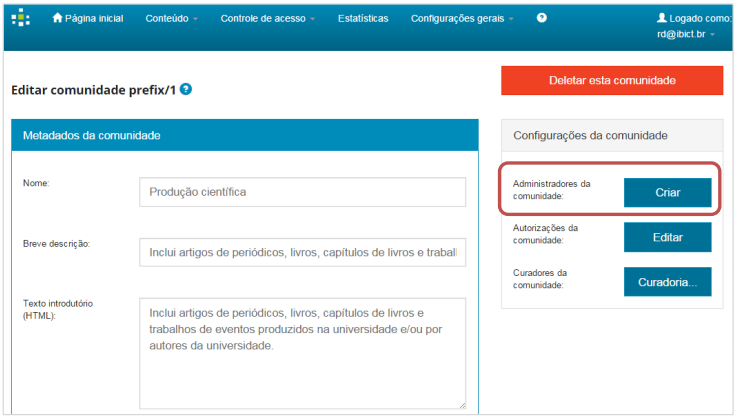
\includegraphics[scale=0.7]{figura/Figura19.png}
                \caption{Criar grupo de administradores da comunidade}
            \label{Rotulo}
        \end{figure}
    
    Passo 3: Para selecionar usuários específicos clique em <Selecionar usuários>.
    
    \begin{figure}[!htp]
                \centering
                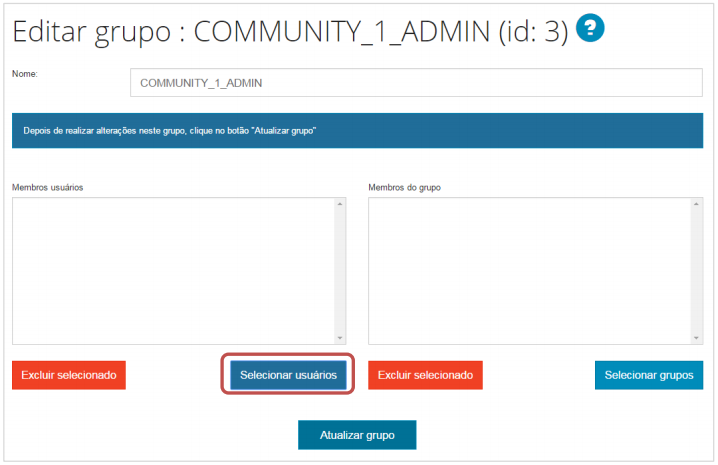
\includegraphics[scale=0.7]{figura/Figura20.png}
                \caption{Selecionar usuários}
            \label{Rotulo}
        \end{figure}
        
\newpage

    Passo 4: Uma lista com todos os usuários já cadastrados no repositório será aberta. Selecione os
    usuários que receberão as permissões de administrador da comunidade e clique em <Adicionar>
    
    \begin{figure}[!htp]
                \centering
                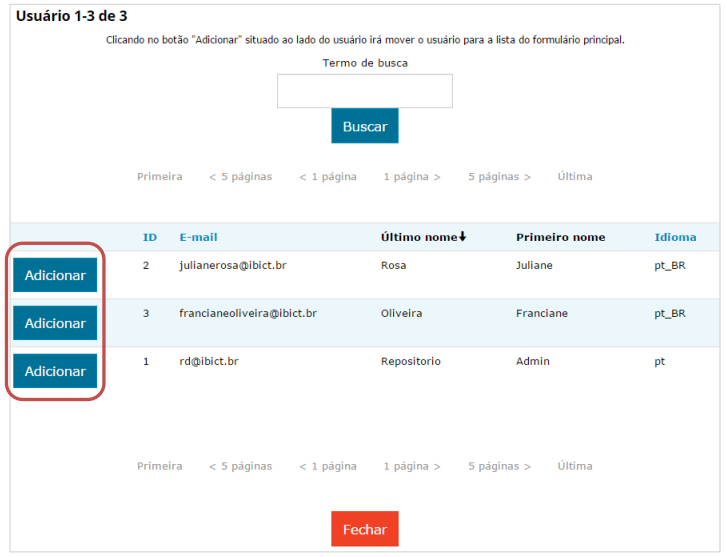
\includegraphics[scale=0.6]{figura/Figura21.png}
                \caption{Selecionar administradores}
            \label{Rotulo}
        \end{figure}
    
    \singlespacing
    Note que é possível navegar pela lista ou realizar uma busca pelo nome dos usuários cadastrados no campo “Termo de busca”.
    \singlespacing
    Passo 5: Após selecionados os usuários, estes deverão aparecer na caixa “Membros usuários”. Para finalizar esta ação clique em <Atualizar grupo>.
    \singlespacing
    \begin{figure}[!htp]
                \centering
                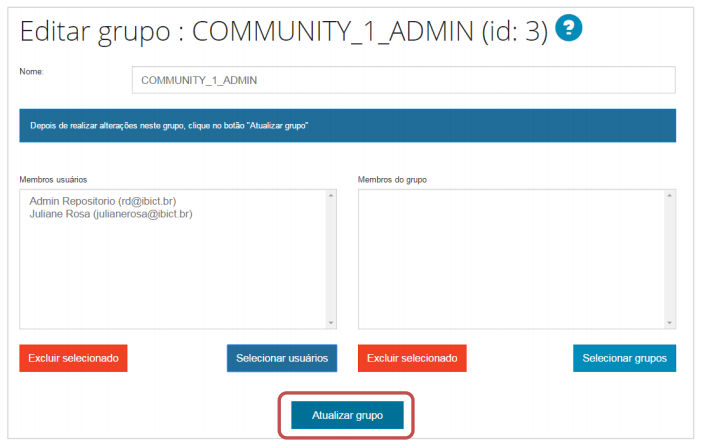
\includegraphics[scale=0.7]{figura/Figura22.png}
                \caption{Atualizar grupo}
            \label{Rotulo}
        \end{figure}

\newpage
    
    Passo 6: Caso queira retirar algum usuário da lista “Membros usuários” da comunidade, selecione o usuário e clique em <Excluir selecionado>.
    
    \begin{figure}[!htp]
                \centering
                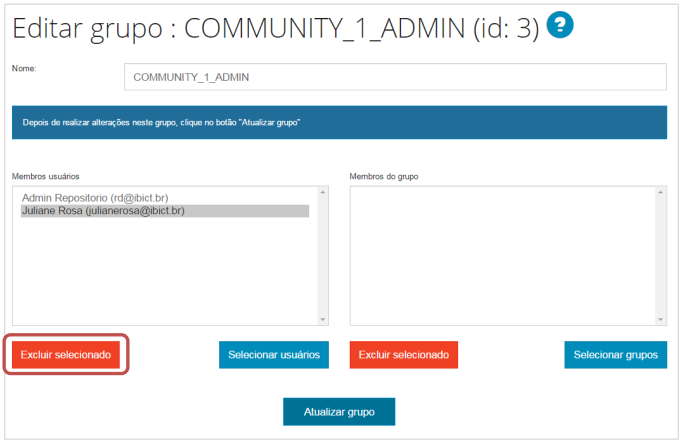
\includegraphics[scale=0.7]{figura/Figura23.png}
                \caption{Excluir membro do grupo}
            \label{Rotulo}
        \end{figure}
        
    Passo 7: O mesmo procedimento para a atribuição de usuários pode ser feito para grupo de usuários. Para tanto, clique em <Selecionar grupos>.
    
    \begin{figure}[!htp]
                \centering
                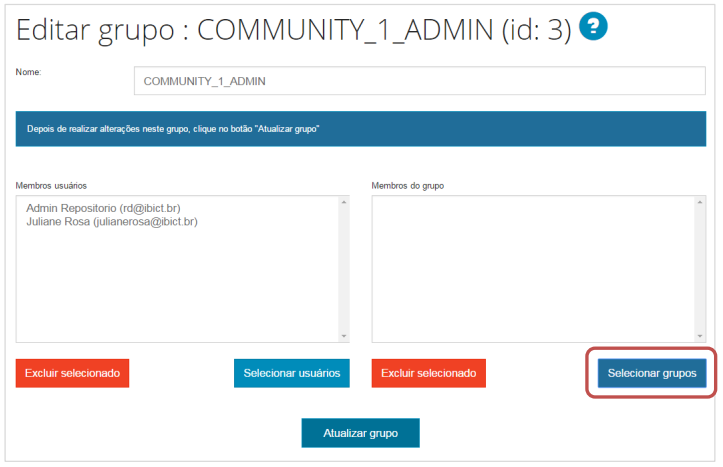
\includegraphics[scale=0.7]{figura/Figura24.png}
                \caption{Grupo de usuários}
            \label{Rotulo}
        \end{figure}

\newpage
    Passo 8: Uma lista com todos os grupos criados será aberta em uma nova janela. Selecione os grupos que receberão as permissões de administrador da comunidade e clique em <Adicionar>.
    
    \begin{figure}[!htp]
                \centering
                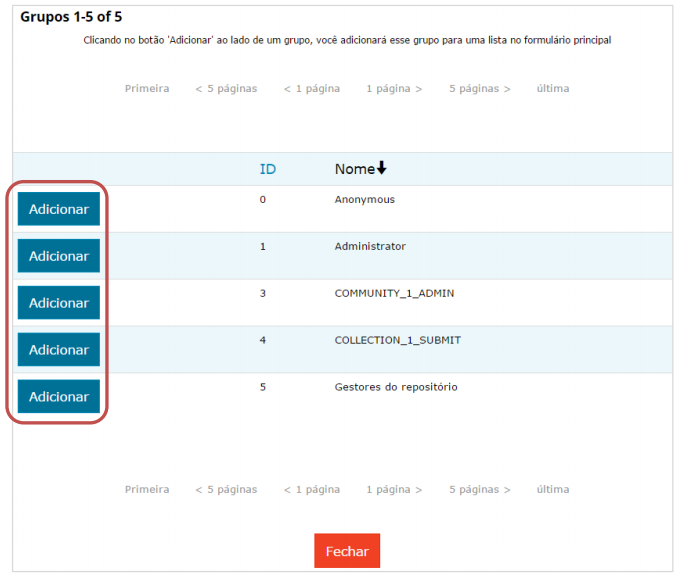
\includegraphics[scale=0.7]{figura/Figura25.png}
                \caption{Permissões aos grupos}
            \label{Rotulo}
        \end{figure}
    
    Passo 9: Depois de selecionado(s) o(s) grupo(s), este(s) deverão aparecer na caixa “Membros do grupo”. Para finalizar esta ação clique em <Atualizar grupo>.
    
    \begin{figure}[!htp]
                \centering
                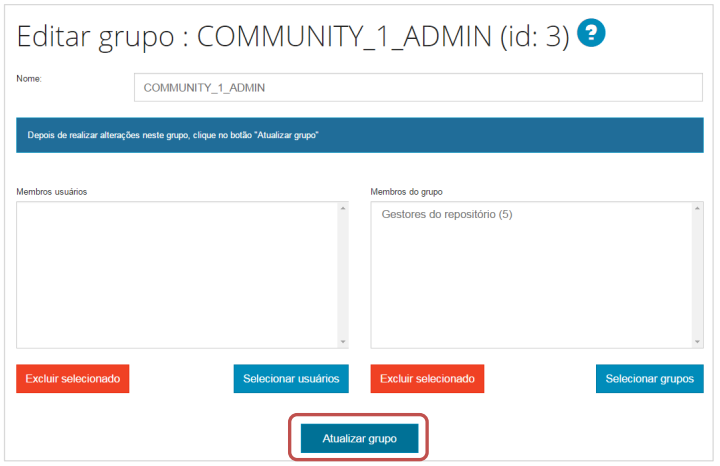
\includegraphics[scale=0.7]{figura/Figura26.png}
                \caption{Confirmar membros do grupo}
            \label{Rotulo}
        \end{figure}
        
\newpage
    Passo 10: Caso queira retirar algum grupo da lista “Membros do grupo” da comunidade, selecione o grupo e clique em <Excluir selecionado>.
    
    \begin{figure}[!htp]
                \centering
                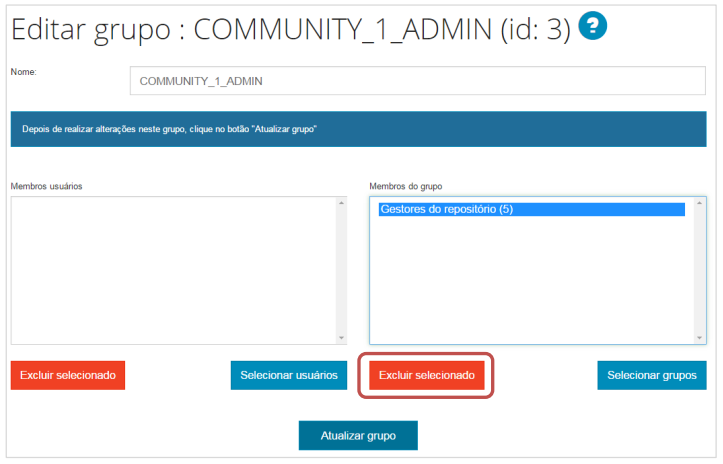
\includegraphics[scale=0.7]{figura/Figura27.png}
                \caption{Excluir membros do grupo}
            \label{Rotulo}
        \end{figure}
        
    Passo 11: Concluída esta etapa, volte para a comunidade para estabelecer suas políticas de funcionamento. Dentro da página <Editar comunidade>, o estabelecimento de políticas de funcionamento será feito na seção “Autorizações da comunidade”, clicando em <Editar>
    
    \begin{figure}[!htp]
                \centering
                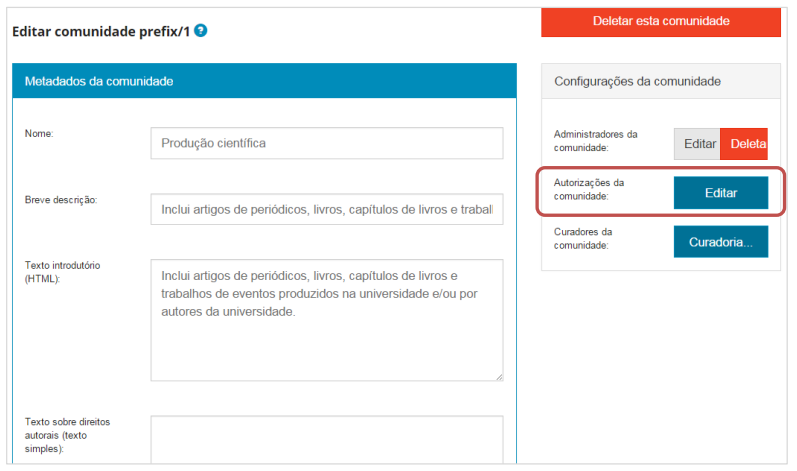
\includegraphics[scale=0.7]{figura/Figura28.png}
                \caption{Estabelecer políticas de funcionamento da comunidade}
            \label{Rotulo}
        \end{figure}
        
\newpage
        
    Passo 12: Para estabelecer uma política diferente da criada automaticamente para a coleção clique em <Adicionar nova política>.
    \singlespacing
    A política criada automaticamente para todas as coleções consiste em permissões de administração do sistema para os usuários pertencentes ao grupo administrador e permissões de navegação e leitura dos documentos depositados na coleção por todos os usuários (Anonymous), exceto dos itens embargados e restritos.
    
    \begin{figure}[!htp]
                \centering
                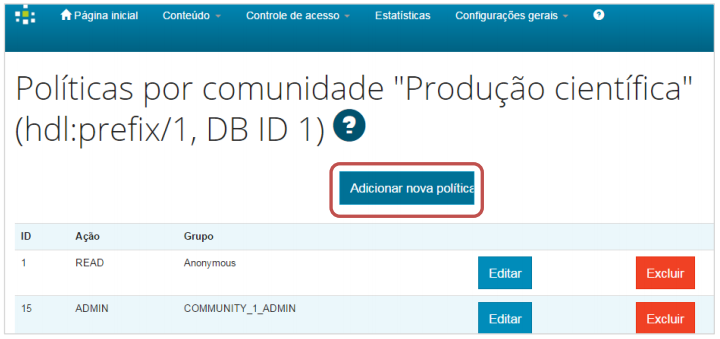
\includegraphics[scale=0.8]{figura/Figura29.png}
                \caption{Estabelecer políticas de funcionamento da comunidade}
            \label{Rotulo}
        \end{figure}
    
    Passo 13: Selecione o grupo de usuários, a permissão que lhe será dada e clique em <Salvar>.
    
    \begin{figure}[!htp]
                \centering
                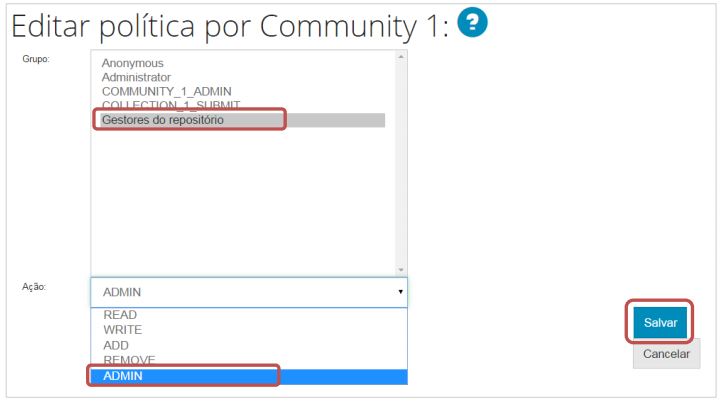
\includegraphics[scale=0.8]{figura/Figura30.png}
                \caption{Editar política por comunidade}
            \label{Rotulo}
        \end{figure}

\newpage
    Informações sobre as permissões:\\
    READ – permissão de visualização/leitura dos registros; \\
    WRITE – permissão de edição dos itens da comunidade;
    ADD – permissão para adicionar/depositar itens dentro da comunidade;
    REMOVE – permissão para remover/excluir itens da comunidade;
    ADMIN – permissão de administrador da comunidade (possui todas as permissões).
    
  \subsection{Criação de subcomunidade}  
  
  Passo 1: Para criar uma subcomunidade, entre em uma comunidade e clique em <Criar subcomunidade>, disponível na caixa de “Ferramentas do administrador”.
  
  \begin{figure}[!htp]
                \centering
                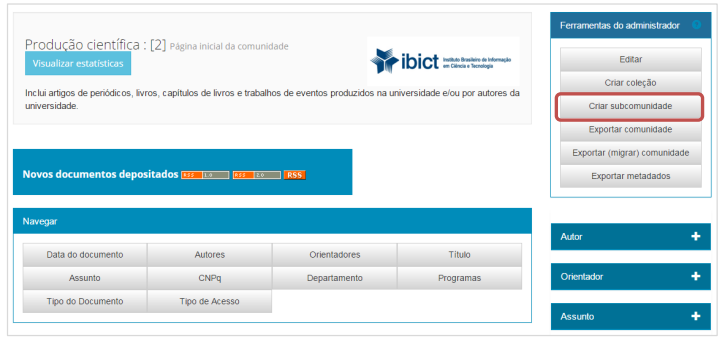
\includegraphics[scale=0.8]{figura/Figura31.png}
                \caption{Criar subcomunidade}
            \label{Rotulo}
        \end{figure}
    
    Passo 2: O processo de criação da subcomunidade é idêntico ao da comunidade. Para acompanhar passo a passo, volte aos itens 3 a 7 da seção 4.1 Criação de comunidade. O processo de estabelecimento de políticas para subcomunidades também é o mesmo das comunidades. A diferença é que você deve acessar a subcomunidade a ser alterada e acessar a respectiva página de edição.
    
    \subsection{Criação de subcomunidade} 
    
    Passo 1: Para editar uma subcomunidade, entre em sua página e clique em <Editar> na caixa de “Ferramentas do administrador”.
    
    \begin{figure}[!htp]
                \centering
                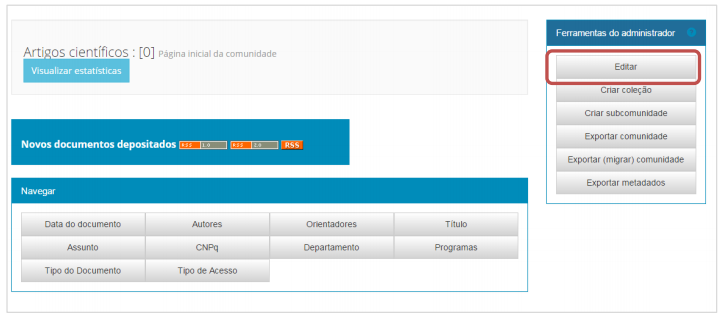
\includegraphics[scale=0.8]{figura/Figura32.png}
                \caption{Criar subcomunidade}
            \label{Rotulo}
        \end{figure}

\newpage  
    \subsection{Criação de coleção}
    
    Passo 1: Para criar uma coleção, entre em uma comunidade ou subcomunidade e clique em <Criar coleção>, nas “Ferramentas do administrador”.
    
    \begin{figure}[!htp]
                \centering
                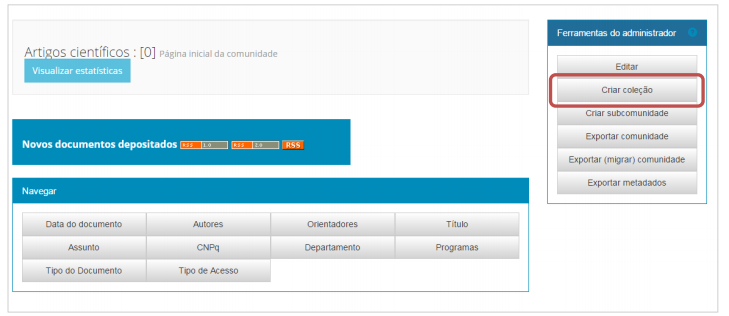
\includegraphics[scale=0.8]{figura/Figura33.png}
                \caption{Criar coleção}
            \label{Rotulo}
        \end{figure}

\newpage
    Passo 2: Descreva a coleção selecionando as características que lhe serão atribuídas. Para selecionar uma característica, basta clicar no quadrado ao lado da frase. Ao finalizar esta fase clique em <Próximo> para continuar o processo de criação da coleção.
    
    \begin{figure}[!htp]
                \centering
                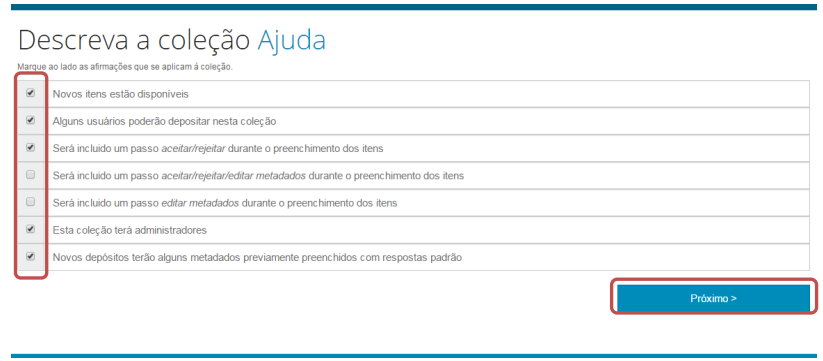
\includegraphics[scale=0.8]{figura/Figura34.png}
                \caption{Descrição da coleção}
            \label{Rotulo}
        \end{figure}
        
    \textbf{\underline{NOTA}}: Essas configurações podem ser editadas posteriormente. 
    
    \singlespacing
    Essas opções formam um fluxo de depósito (workflow) no repositório. Isso significa que elas incluem ou excluem etapas no processo de depósito, que podem ser atribuídas a pessoas diferentes, com permissões diferentes.
    \singlespacing
    
    \textbf{Novos itens estão disponíveis}: os itens inseridos nessa coleção poderão ser visualizados (READ) por usuários anônimos (grupo: Anonymous), ou seja, o padrão para a coleção é ter seus documentos disponíveis ao público, com exceção dos itens restritos e embargados. Se esta opção não estiver marcada, será necessário definir os usuários específicos (ou grupos de usuários) que terão acesso aos itens dessa coleção.
    
    \singlespacing
    
    \textbf{Alguns usuários poderão depositar nesta coleção}: você deverá selecionar quais usuários poderão fazer depósitos nessa determinada coleção. Se esta opção não for marcada ou se nenhum usuário for selecionado, apenas usuários com perfil de administrador poderão realizar o depósito
    
    \singlespacing
    
    \textbf{Será incluído um passo aceitar/rejeitar durante o preenchimento dos itens}: inclui a etapa de avaliação no processo de depósito. Após os usuários depositantes realizarem a submissão de um item, ele não ficará automaticamente disponível no repositório. É preciso que o administrador ou outro usuário/grupo determinado aprove o depósito. Quando esta opção é marcada, é preciso definir os usuários ou grupos responsáveis por aprovar ou rejeitar um depósito. Esses usuários terão acesso ao registro feito pelo depositante e poderão visualizar os metadados preenchidos. Terão a opção de aprovar o depósito (enviando-o para a próxima etapa do fluxo, se houver, ou tornando-o disponível) ou rejeitar o depósito (envia mensagem ao depositante sobre motivo da não aprovação).
    
    \singlespacing
    
    \textbf{Será incluído um passo aceitar/rejeitar/editar metadados durante o preenchimento dos itens}: funciona da mesma maneira que a opção anterior, mas além do usuário responsável pela revisão poder “aprovar” e “rejeitar” um depósito, ele poderá também alterar os seus metadados. Se houver erros a serem corrigidos no depósito, o próprio revisor poderá consertá-los, em vez de solicitar que o depositante os conserte.
    
\newpage
    
    \textbf{Será incluído um passo editar metadados durante o preenchimento dos itens}: novamente, tem o mesmo funcionamento das opções anteriores. É preciso selecionar um usuário ou grupo responsável por revisar os depósitos realizados na coleção. Esses usuários terão a opção de alterar os metadados desse depósito. Após revisar e editar os metadados desejados, os responsáveis podem completar e disponibilizar o depósito, ou seja, tornar o registro disponível para o público.
    
    \singlespacing
    
    \textbf{Esta coleção terá administradores}: caso deseje selecionar usuários específicos para administrarem uma determinada coleção, marque essa opção. Esta opção pode ser usada, por exemplo, para dar autonomia para cada campus da universidade ou para cada faculdade/instituto gerenciar a sua coleção.
    
    \singlespacing
    
    \textbf{Novos depósitos terão alguns metadados previamente preenchidos com respostas padrão}: você pode determinar que certos metadados de uma coleção específica sejam preenchidos sempre com os mesmos valores. Por exemplo, em uma coleção que só receberá artigos científicos, você pode pré-determinar o metadado que registra o tipo de documento como “artigo de periódico” para todos os itens dessa coleção.
    
    \singlespacing
    
    A configuração do fluxo de depósito é explicada no tópico 3.3.2 Estabelecimento de políticas e fluxo de depósito da coleção. 
    
    \singlespacing
    
    Passo 3: Preencha os campos que julgar necessários para descrever a coleção e clique em <Próximo>.
    
    \begin{figure}[!htp]
                \centering
                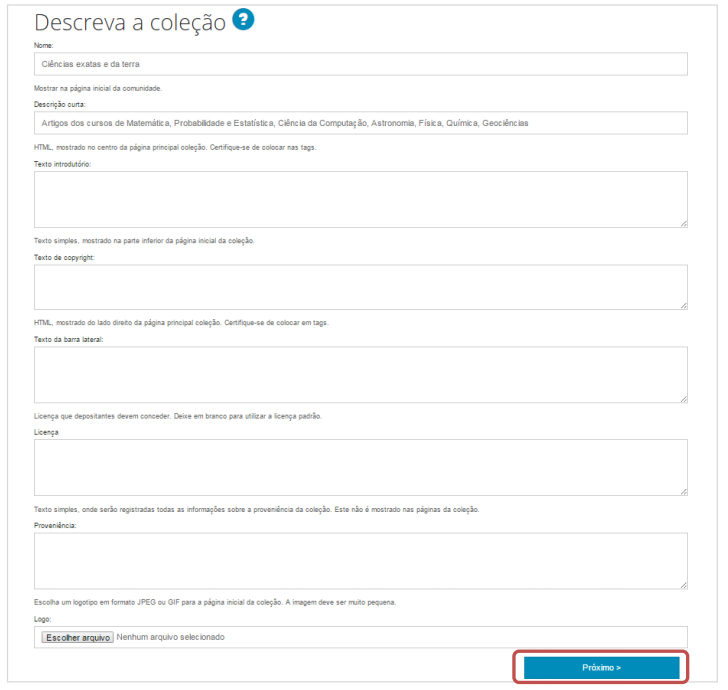
\includegraphics[scale=0.7]{figura/Figura35.png}
                \caption{Descrever a coleção}
            \label{Rotulo}
        \end{figure}

\newpage

    \singlespacing 
     
    \textbullet \hspace{6pt} \textbf{Nome}: informe o nome que será dado à coleção. Exemplo: Ciências exatas e da terra.
     
    \singlespacing
     
    \textbullet \hspace{6pt} \textbf{Descrição curta}: descreva a coleção. Exemplo: Artigos dos cursos de Matemática, Probabilidade e Estatística, Ciência da Computação, Astronomia, Física, Química, Geociências.
    
    \singlespacing
     
    \textbullet \hspace{6pt} \textbf{Texto introdutório (HTML)}: insira um texto sobre a coleção. Permite o uso de tags html que alteram a apresentação do texto. Exemplo: <p><b> Coleção de artigos 34 publicados por alunos e docentes dos cursos de Matemática, Probabilidade e Estatística, Ciência da Computação, Astronomia, Física, Química, Geociências. </b> </p>
    
    \singlespacing
     
    \textbullet \hspace{6pt} \textbf{Texto de copyright}: utilizado para informar os usuários sobre os direitos do autor. É um campo meramente informativo, implica num aviso, estando em conformidade com a política de acesso e de preservação da instituição mantenedora do repositório. Pode ser utilizado para explicar a restrição em coleções de acesso controlado, por exemplo.
    
    \singlespacing
     
    \textbullet \hspace{6pt} \textbf{Texto da barra lateral}: insira outro texto que queira para descrever a comunidade que aparecerá na barra lateral da página da comunidade.
    
    \singlespacing
     
    \textbullet \hspace{6pt} \textbf{Proveniência}: não aparece na página da coleção. Esse campo pode ser utilizado para inserir outras informações relevantes à coleção, sendo que apenas o administrador terá acesso a essas informações no processo de edição da coleção. É utilizado para indicar a origem dos documentos depositados em determinada coleção.
    
    Passo 4: Se anteriormente você marcou a opção “Alguns usuários poderão depositar nesta coleção”, o próximo passo é a atribuir autorização para o depósito de documentos na coleção, ou seja, selecionar os usuários que poderão adicionar itens a essa coleção.
    
    Clique em <Selecionar usuários> para selecionar usuários individualmente ou <Selecionar grupos> para selecionar grupos de usuários previamente estabelecidos. Após a seleção clique em <Próximo>.
    
    \begin{figure}[!htp]
                \centering
                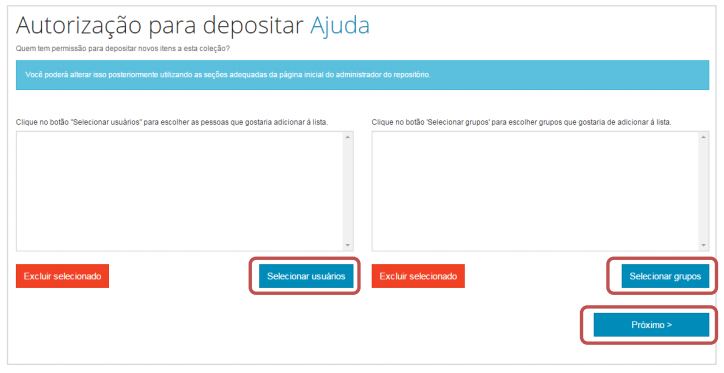
\includegraphics[scale=0.8]{figura/Figura36.png}
                \caption{Permissões de depósito na coleção}
            \label{Rotulo}
        \end{figure}

\newpage

    Passo 5: Se anteriormente você marcou a opção “Esta coleção terá administradores”, o próximo passo é selecionar os usuários ou grupo de usuários que terão permissão de administrador da coleção. Após selecioná-los, clique em <Próximo>
    
    \begin{figure}[!htp]
                \centering
                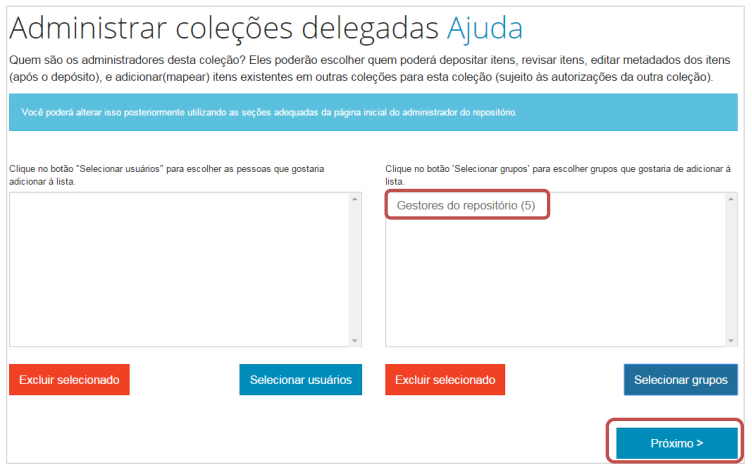
\includegraphics[scale=0.7]{figura/Figura37.png}
                \caption{Permissões de administrador da coleção}
            \label{Rotulo}
        \end{figure}
    
    Passo 6: Se anteriormente você marcou a opção “Novos depósitos terão alguns metadados previamente preenchidos com respostas padrão”, o próximo passo é configurar os campos que terão valores pré-definidos dentro da coleção.
    
    \singlespacing
    
    Escolha o metadado nas caixas de seleção. Insira o valor do campo, ou seja, como ele será preenchido, e a sigla do idioma, de acordo com o padrão adotado. A seguir, clique em Próximo.
    
    \begin{figure}[!htp]
                \centering
                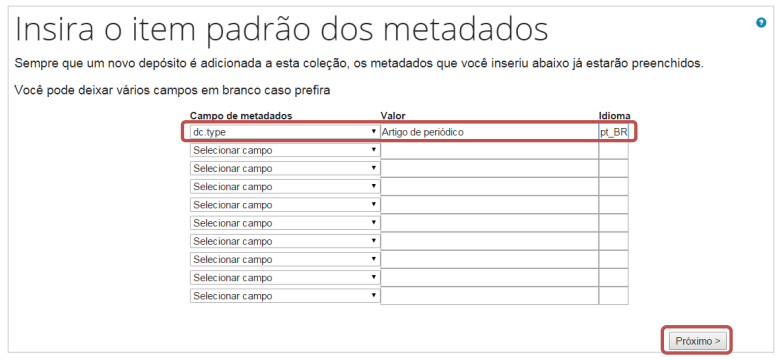
\includegraphics[scale=0.7]{figura/Figura38.png}
                \caption{Configurar metadados pré-definidos}
            \label{Rotulo}
        \end{figure}
        
\newpage

    Passo 7: Finalizada esta etapa, a coleção está criada. A próxima tela que aparecerá é de edição
    da coleção. Nesta tela, é possível alterar todas as informações inseridas nas etapas anteriores ou incluir novas informações. Clique em <Atualizar> para confirmar as alterações.
    
    \begin{figure}[!htp]
                \centering
                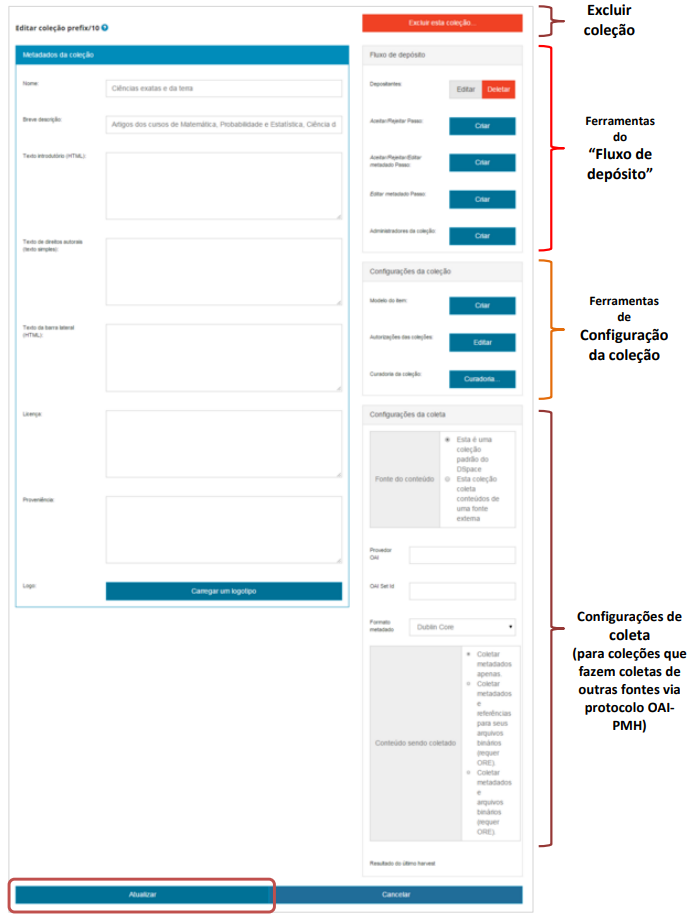
\includegraphics[scale=0.9]{figura/Figura39.png}
                \caption{Página de edição da coleção}
            \label{Rotulo}
        \end{figure}
    
\newpage

    \subsection{Editar coleção}
    
    Passo 1: Para editar as configurações de uma coleção, entre na página da mesma e clique em <Editar>, disponível na caixa de “Ferramentas do administrador”.
        
    
    
    
    
    
    
    
    
    
    

    
    
    
    
    
    
    
    

    
    

    
    
    
    
    
    
    
    
    
    
    
    
    
    
    
    
    
     
     

        

    
        
        
        
        
        
        
        
        
        
        
        
\newpage
        \subsection{O que é o DSpace?} 
        Para que serve?
        DSpace é um software de código-fonte aberto que fornece facilidades para o gerenciamento de acervo digital, utilizado para implementação de repositórios institucionais. Suporta uma grande variedade de tipo de documentos, tais como: livros, teses e dissertações, fotografias, filmes, áudio, e outros. Os documentos são organizados em comunidades e coleções.
        O DSpace é disponibilizado livremente às instituições de investigação, sob a forma de um produto de código aberto, que pode ser livremente adaptado e expandido funcionalmente, nos termos da Licença BSD Open source licensx

    \subsection{Especificações técnicas do sistema}
        A Recomendação mínima recomendada para um pequeno servidor:
        
    \singlespacing \textbullet \hspace{6pt} 2 GB de memória RAM
 
    \textbullet \hspace{6pt} 40 GB de disco rígido
 
    \textbullet \hspace{6pt} Placa de rede on-board
 
    \textbullet \hspace{6pt} Processador de único núcleo, com 2.6 GHz

    \singlespacing  O DSpace utiliza os seguintes software para operar um servidor e cada um deles utiliza uma política de uso da documentação específica. Abaixo segue uma lista com os software: 
 
    \singlespacing \textbullet \hspace{6pt} Apache Ant, http://ant.apache.org/manual/index.html
  
    \textbullet \hspace{6pt} Apache Maven 3.0.5 ou superior (3.3.9 +), https://maven.apache.org/index.html
  
    \textbullet \hspace{6pt} Apache Tomcat 7 ou 8, http://tomcat.apache.org/
 
    \textbullet \hspace{6pt} JDK 7 ou 8(64-bit) http://openjdk.java.net/install/

\newpage
\section{Instalação}
\newpage
\begin{enumerate}
    
    \item \textbf{Crie o usuário do DSpace:} 
    
        \begin{minted}{bash}
useradd -m dspace
        \end{minted}
    
        \begin{minted}{bash}
passwd dspace
        \end{minted}
    
   
    \item \textbf{Execute a atualização dos pacotes do seu sistema operacional:} 
    
        \begin{minted}{bash}
apt-get update && apt-get upgrade -y
        \end{minted}
   
    \item \textbf{Instale o Oracle-JDK}
        \begin{enumerate}
            \item O Java Development Kit (JDK), promove portabilidade das aplicações desenvolvidas nessa linguagem. Existem versões open source dessa ferramenta, como o Open-JDK, no entanto a compilação e execução do DSpace 6.x funciona com as versões Oracle-JDK 1.7.x e Oracle-JDK 1.8.x. Esta não é uma versão livre, mas ao aceitar sua licença, há a liberação do download, sem custos para o usuário. A Oracle-JDK 1.8.x pode ser baixada no seguinte endereço:
            \singlespacing
            https://www.oracle.com/technetwork/java/javase/downloads/jdk8-downloads-2133151.html
            
            \begin{minted}{bash}
mkdir /opt/jdk
        \end{minted}
        
        \begin{minted}{bash}
tar -zxf jdk-8u221-linux-x64.tar.gz -C /opt/jdk
        \end{minted}
        
        \item Feito isso, deve-se instalar o pacote, o que pode ser efetuado, estando ainda logado como root, por meio dos comandos:
        
        \begin{minted}{bash}
update-alternatives --install /usr/bin/java java /opt/jdk/jdk1.8.0_221/bin/
java 100
        \end{minted}
        
        \begin{minted}{bash}
update-alternatives --install /usr/bin/javac javac /opt/jdk/jdk1.8.0_221/bin/
javac 100
        \end{minted}

        \end{enumerate}
     
        
    \item \textbf{Instale o Apache Maven 3.0.5 ou superior (3.3.9 +) * (ferramenta de compilação Java)}\\
        \begin{enumerate}
            \item O Apache-Maven é a ferramenta que realiza a construção de toda a árvore de pacotes que serão necessários para instalação do DSpace, e além disso compila o código fonte, deixando-o pronto para instalação. Para a instalação do Apache-Maven, deve-se baixar o seu pacote binário no endereço http://maven.apache.org/ e descompactá-lo, estando dentro da /home/dspace/ por meio do comando (x.x.x representa o número da versão baixada):
        \end{enumerate}
        
            \texttt{tar -vzxf apache-maven-x.x.x-bin.tar.gz}\\
        
        
    \item \textbf{ Instale o Apache Ant 1.8 ou posterior (ferramenta de compilação Java)}\\
         \begin{enumerate}
            \item A ferramenta que executa a tarefa de instalação do DSpace é o Apache-Ant. Para tornar esse software disponível para uso, basta realizar o download de seu pacote binário em http://ant.apache.org/ e descompactá-lo dentro da /home/dspace.\\
            
                \texttt{tar -vzxf apache-ant-x.x.x-bin.tar.gz}\\
            
            \item \textbf{Ou então se preferir, execute:}\\
                \begin{minted}{bash}
apt-get install ant
                \end{minted}
            
        \end{enumerate}
        
        \item \textbf{Instale o Apache-Tomcat, é o servidor Web que torna disponível o acesso do DSpace via rede (seja a Intranet ou a Internet).} \\
    
        
        \begin{enumerate}
            \item Para instalá-lo basta baixar seu pacote binário em http://tomcat.apache.org/ e descompactá-lo dentro da /home/dspace. (O Tomcat 8.0.32 encontrado, por exemplo, no Debian 9 Stretch e Ubuntu 16.04 Xenial ) tem um bug que causará PropertyBatchUpdateException ou StringIndexOutOfBoundsException.   Isto foi corrigido em 8.0.33. Se você estiver usando o Tomcat 7, recomendamos executar o Tomcat 7.0.30 ou superior. Tomcat 7.0.29 e versões inferiores sofrem um vazamento de memória. Como resultado, essas versões do tomcat requerem uma quantidade incomum de memória para executar o DSpace. Isso foi resolvido a partir do Tomcat 7.0.30.)
        \end{enumerate}
        
                \texttt{tar -vzxf apache-tomcat.xxxx.tar.gz} \\
        
        \item \textbf{Baixe o DSpace customizado pelo IBICT do GitHub e jogue no diretório do dspace:}\\
        
            \texttt{cd /home/dspace/}\\
        
        \item \textbf{Descompacte o arquivo:}\\
        
            \texttt{unzip repositorio-padrao-dspace-6\_\textbf{x}.zip}\\
            
        \item \textbf{Instale o Git (na verdade não é usado com este método, mas resolve um erro produzido pelo maven):}\\    
            
            \begin{minted}{bash}
apt-get install git
            \end{minted}
            
        \item \textbf{Instale o PostgreSQL 9.6: (versões anteriores do PostgreSQL <9.4 podem não funcionar corretamente com o DSpace, por causa da extensão do pgcrypto):}\\
            
        \begin{minted}{bash}
sh -c 'echo "deb http://apt.postgresql.org/pub/repos/apt/ 
`lsb_release -cs`-pgdg main" >> /etc/apt/sources.list.d/pgdg.list'
        \end{minted}

       \begin{minted}{bash}
wget -q https://www.postgresql.org/media/keys/ACCC4CF8.asc -O - | apt-key add -
       \end{minted}
      
       \begin{minted}{bash}
apt-get update
       \end{minted}
            
        \begin{minted}{bash}
apt-get install postgresql-9.6 postgresql-contrib-9.6
       \end{minted}


        \item \textbf{Vamos fazer o login no PostgreSQL e criar o banco de dados e o usuário do banco de dados do DSpace:}\\
        
            \begin{minted}{bash}
su - postgres
            \end{minted}
            
            \begin{minted}{bash}
createuser --username=postgres --no-superuser --pwprompt dspace
            \end{minted}
            
            \begin{minted}{bash}
createdb --username=postgres --owner=dspace --encoding=UNICODE dspace
            \end{minted}
            
            \begin{minted}{bash}
psql --username=postgres dspace -c "CREATE EXTENSION pgcrypto;"
            \end{minted}
            
             \begin{minted}{bash}
exit
            \end{minted}
            
        \item \textbf{Agora devemos adicionar uma linha ao PostgreSQL para autenticação do cliente:}\\
    
        \begin{enumerate}
            \item Abra o arquivo pg\_hba.conf com seu editor favorito (nano, vi, etc.)\\
            
                \texttt{nano /etc/postgresql/9.6/main/pg\_hba.conf}\\

            \item E adicione a seguinte linha\\
            
                \texttt{local     all     dspace    md5}\\
                
             \item Reinicie o PostgreSQL para adotar as mudanças\\
            
                \texttt{/etc/init.d/postgresql restart}\\

            \end{enumerate}
            
        \item \textbf{Certifique-se que o diretório destino de instalação está com permissões de escrita ao usuário dspace, deve-se logar como root e executar o comandos:}\\
        
            \texttt{mkdir /dspace-base}
            
             \begin{minted}{bash}
chown -R dspace:dspace /dspace-base/
            \end{minted}
            
            \begin{minted}{bash}
chown -R dspace:dspace /home/dspace/
            \end{minted}
            
        \item \textbf{Todos comandos a seguir devem ser executados com o usuário dspace, salvo se explicitado o login de root.}\\
        
        \item \textbf{Entre na pasta DSpace-fonte.  Será necessário que se realize uma cópia do local.cfg EXAMPLE para local.cfg. Localizado em: DSpace/config/local.cfg.exemple.}\\
        
            \texttt{cp local.cfg.EXAMPLE local.cfg}\\
            
        \item \textbf{Não esqueça de entrar no arquivo local.cfg. E Preencher o campo do dspace.install.dir como dspace-base}\\
            
            \texttt{dspace.install.dir=/dspace-base}\\
        
        \item \textbf{Comandos para executar o maven:}\\
        
            \texttt{cd repositorio-padrao-dspace-6\_x/}\\
            
             \begin{minted}{bash}
/home/dspace/apache-maven-x.x.x/bin/mvn -U package
            \end{minted}
            
            \begin{enumerate}
            \item Após aproximadamente 30 min, o sistema deve responder com um log na tela, e ao final a mensagem BUILD SUCCESSFUL.\\

            \end{enumerate}
            
        \item \textbf{O próximo é o apache Ant:}\\
        
         \begin{enumerate}
            \item Caso tenha baixado o pacote binário. Com o usuário dspace, a instalação deve ser executada dentro do DSpace-fonte/dspace/target/dspace-installer, e é realizada por meio do comando.\\
            
                \begin{minted}{bash}
/home/dspace/apache-ant-x.x.x/bin/ant fresh_install\\
            \end{minted}
            
            \item Se tiver baixado o pacote pelo apt-get install ant, siga os seguintes passos:\\
            
            \texttt{cd dspace/target/dspace-installer}\\
            
            \begin{minted}{bash}
ant fresh_install
            \end{minted}

            \end{enumerate}
            
        \item \textbf{Finalizada a instalação do apache-Ant. Faça as modificações necessárias no arquivo dspace.cfg. Localizado em /dspace-base/config. Este arquivo é composto dos parâmetros de configuração do dspace. Segue uma tabela descritiva dos principais variáveis a serem configuradas:}
            
        \begin{figure}[!ph]
            \centering
            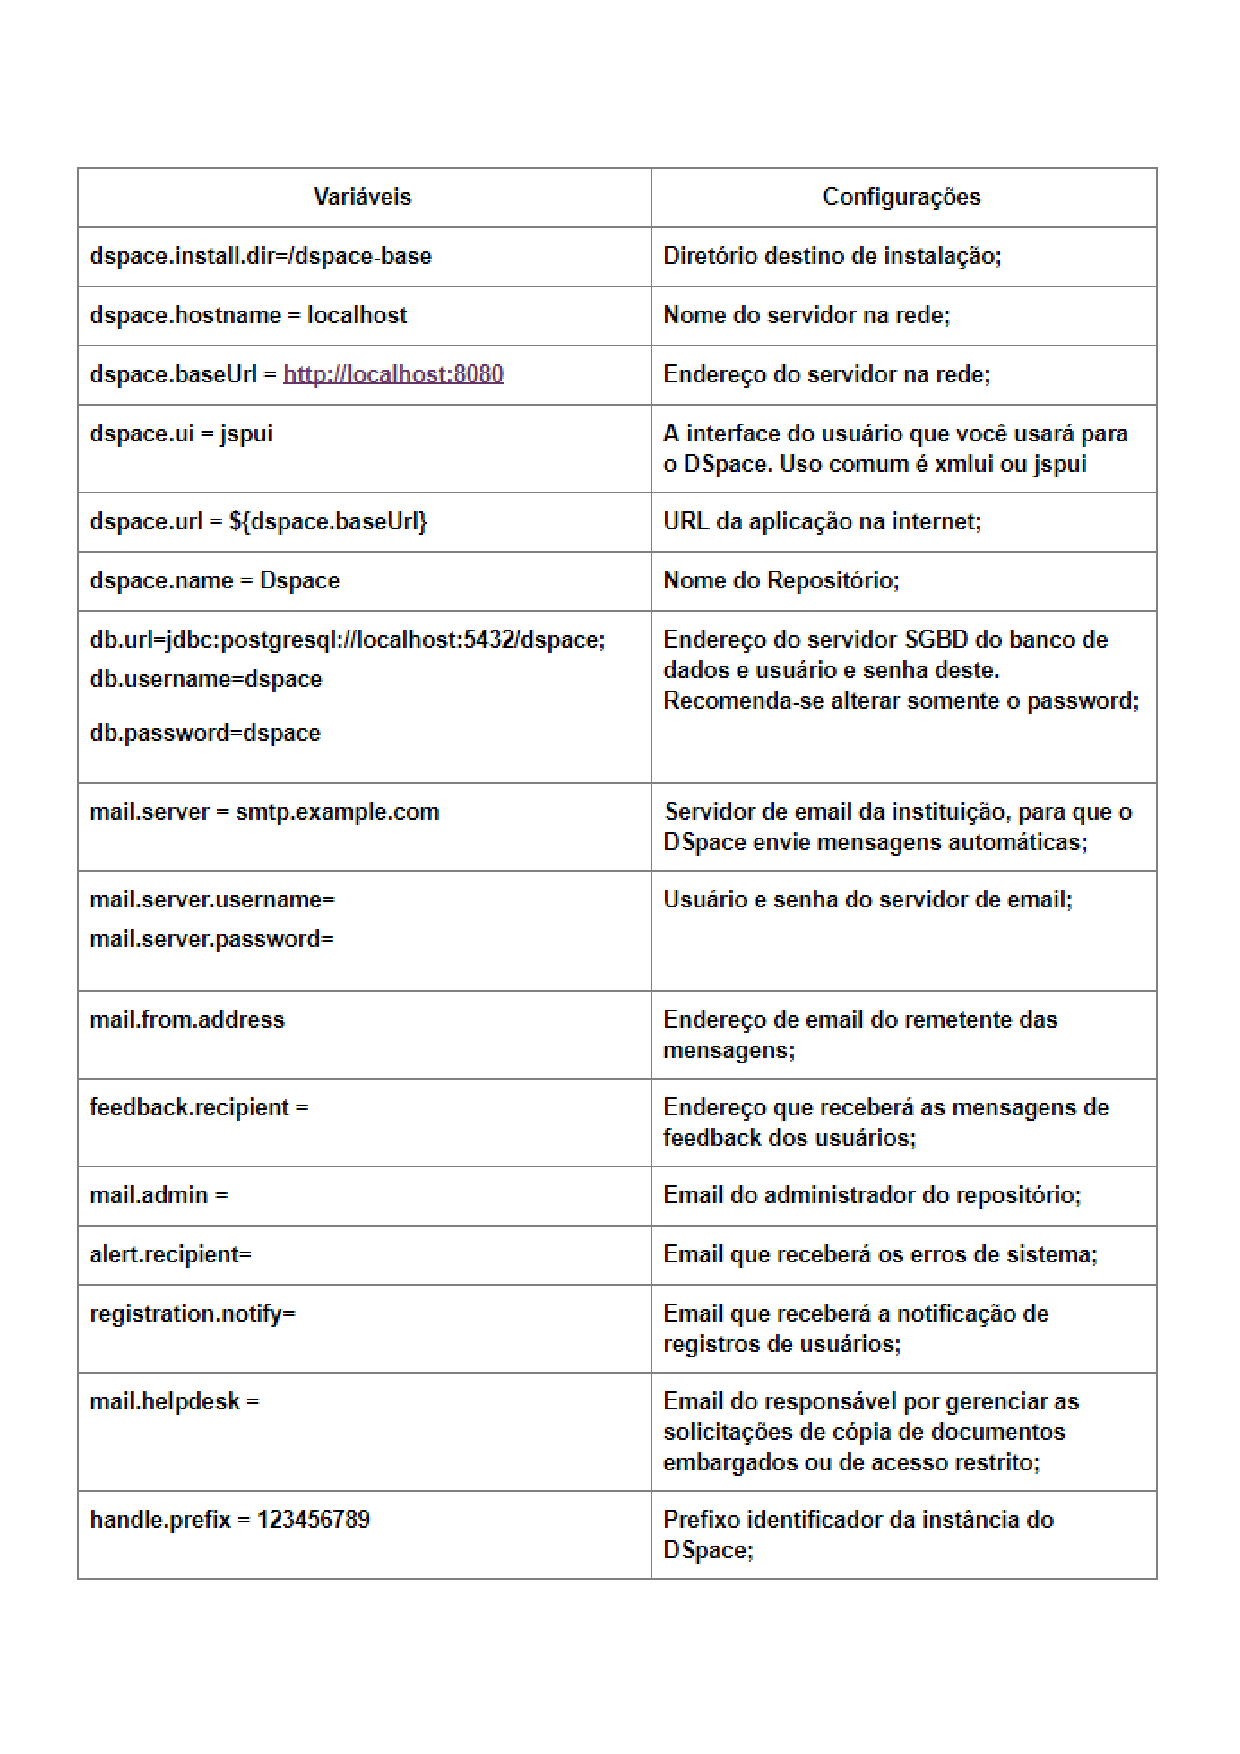
\includegraphics[scale=0.7]{figura/variaveis.pdf}
            \caption{Tabela das configurações básicas.}
        \label{Rotulo}
        \end{figure}
        
        
        \newpage

        \item \textbf{Finalizada a instalação do apache-Ant. Faça as modificações necessárias no arquivo dspace.cfg. Localizado em /dspace-base/config. Este arquivo é composto dos parâmetros de configuração do dspace. Segue uma tabela descritiva dos principais variáveis a serem configuradas:}
        
            \texttt{<Connector port="8080" protocol="HTTP/1.1"\\
                    connectionTimeout="20000"\\
                    redirectPort="8443" URIEncoding="UTF-8" />}\\
            
        
        \item \textbf{A ativação do servidor Web Apache-Tomcat com a aplicação do DSpace se dá por meio dos comandos. E deve ser executada dentro encontra /dspace-base/webapps:}\\
            
         \begin{minted}{bash}
cp -R jspui/ solr/ oai/  /home/dspace/apache-tomcat-x.x.x/webapps/
         \end{minted}
         
          \item \textbf{Este último expande os parâmetro de memória reservada para o Apache-Tomcat. Contudo, se o servidor for reiniciado, essa configuração será perdida. Para torná-la definitiva, edite o arquivo que se encontra em home/dspace/apache-tomcat-x.x.x/bin/catalina.sh e adicione ao final dele as linhas:}\\
          
            \begin{minted}{bash}
JAVA_OPTS="-Djava.awt.headless=true -Xms512M -Xmx768M -XX:MaxPermSize=256M 
-XX:+UseParallelGC -XX:MaxGCPauseMillis=1500 -XX:GCTimeRatio=9 -server
-XX:+DisableExplicitGC"
            \end{minted}
         
         \item \textbf{Por fim, com o usuário dspace basta que se inicie o servidor Apache-Tomcat:}\\

            \begin{minted}{bash}
/home/dspace/apache-tomcat-x.x.x/bin/startup.sh
            \end{minted}
            
        \item \textbf{Em seguida, crie o administrador do DSpace. Após a instalação do DSpace é necessário que se crie uma senha de administrador, o que pode ser feito pelo comando:}\\
        
            \begin{minted}{bash}
/dspace-base/bin/dspace create-administrator
            \end{minted}
            
        \item \textbf{Agora você pode acessar a página principal do DSpace JSPUI em:}\\
        
        \begin{minted}{bash}
http://localhost:8080/jspui
            \end{minted}

\end{enumerate}

\newpage
\section{Configurações básicas}
\newpage
      \subsection{Protocolo oai}
 
      É por meio do protocolo OAI-PMH que é feita a coleta dos Repositórios, Bibliotecas e Revistas para o Portal brasileiro de publicações científicas em acesso aberto (oasisbr) <http://oasisbr.ibict.br/vufind/>  e a Biblioteca Digital Brasileira de Teses e Dissertações (BDTD) <http://bdtd.ibict.br/vufind/>. Devem ser feito os devidos apontamentos neste arquivo para o perfeito funcionamento da url de coleta.\\
      
      Localizado em \textbf{/dspace-base/config/modules/oai.cfg} 

          \begin{figure}[!htp]
                \centering
                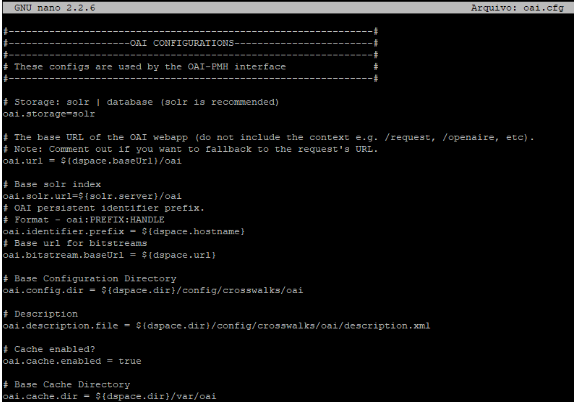
\includegraphics[scale=0.9]{figura/oai.png}
                \caption{Arquivo oai.cfg.}
            \label{Rotulo}
          \end{figure}
        
    \subsection{Ativação da url oai}
   
    Em sua instalação padrão, o OAI está disponível dentro da pasta \textbf{[dspace-base]/webapps/oai/} da instalação do DSpace. E para sua ativação, deve-se seguir os seguintes passos:
        
        
        \begin{enumerate}
            \item Copiar as pastas \textbf{[dspace-base]/webapps/oai/} e \textbf{[dspace-base]/webapps/solr/} para dentro da webapps, do servidor de aplicação Apache-Tomcat;
            
            \item Reiniciar o servidor Apache-Tomcat;
            
            \item Executar o comando:\\
             \texttt{[dspace-base]/bin/dspace oai import -c -v}\\
             \texttt{[dspace-base]/bin/dspace oai clean-cache}

        \end{enumerate}
        
\newpage
    \subsection{Sincronização automática da url OAI do repositório}
    Ainda é necessário que se inclua alguns comandos na \textbf{contrab} do sistema, que é uma forma de agendar algumas tarefas que deverão ser executadas durante o período em que o uso do sistema pela comunidade não seja tão intenso. Esse procedimento pode ser efetuado, quando se está logado como root, se executa o comando: \textbf{crontab -e}. Após abertura do arquivo da crontab, devem ser adicionadas as seguintes linhas, informando o usuário dspace, os caminhos e os comandos no final do documento:
    
    \begin{minted}{bash}
0 0 * * * dspace /dspace-base/bin/dspace oai import
    \end{minted}

\newpage
\section{Formulário de entrada}
\newpage
    \subsection{O que é o Formulário de entrada?}
O formulário de entrada é utilizado para determinar a estrutura dos metadados que serão usados para descrever os documentos durante o processo de submissão.
\singlespacing
Em linguagem mais simples e no contexto dos repositórios, os metadados são os campos que serão preenchidos para descrever o objeto digital que está sendo submetido.
É um arquivo em XML (eXtensible Markup Language) composto por campos (indicados pela tag <field>) que podem ser adequados aos tipos de documentos contidos no repositório, ou seja, você pode configurar o formulário para que este contenha os metadados necessários de acordo com o tipo de documento a ser depositado.
\singlespacing
Essa configuração não pode ser feita através da interface gráfica, sendo necessário o auxílio de equipe com conhecimento técnico do DSpace para que seja executada.
O endereço do arquivo que permite a edição do formulário é o \textbf{[dspace-base]/config/input-forms.xml}. Para registrar novos metadados no DSpace é necessário inseri-los também via interface.

        \begin{figure}[!htp]
                \centering
                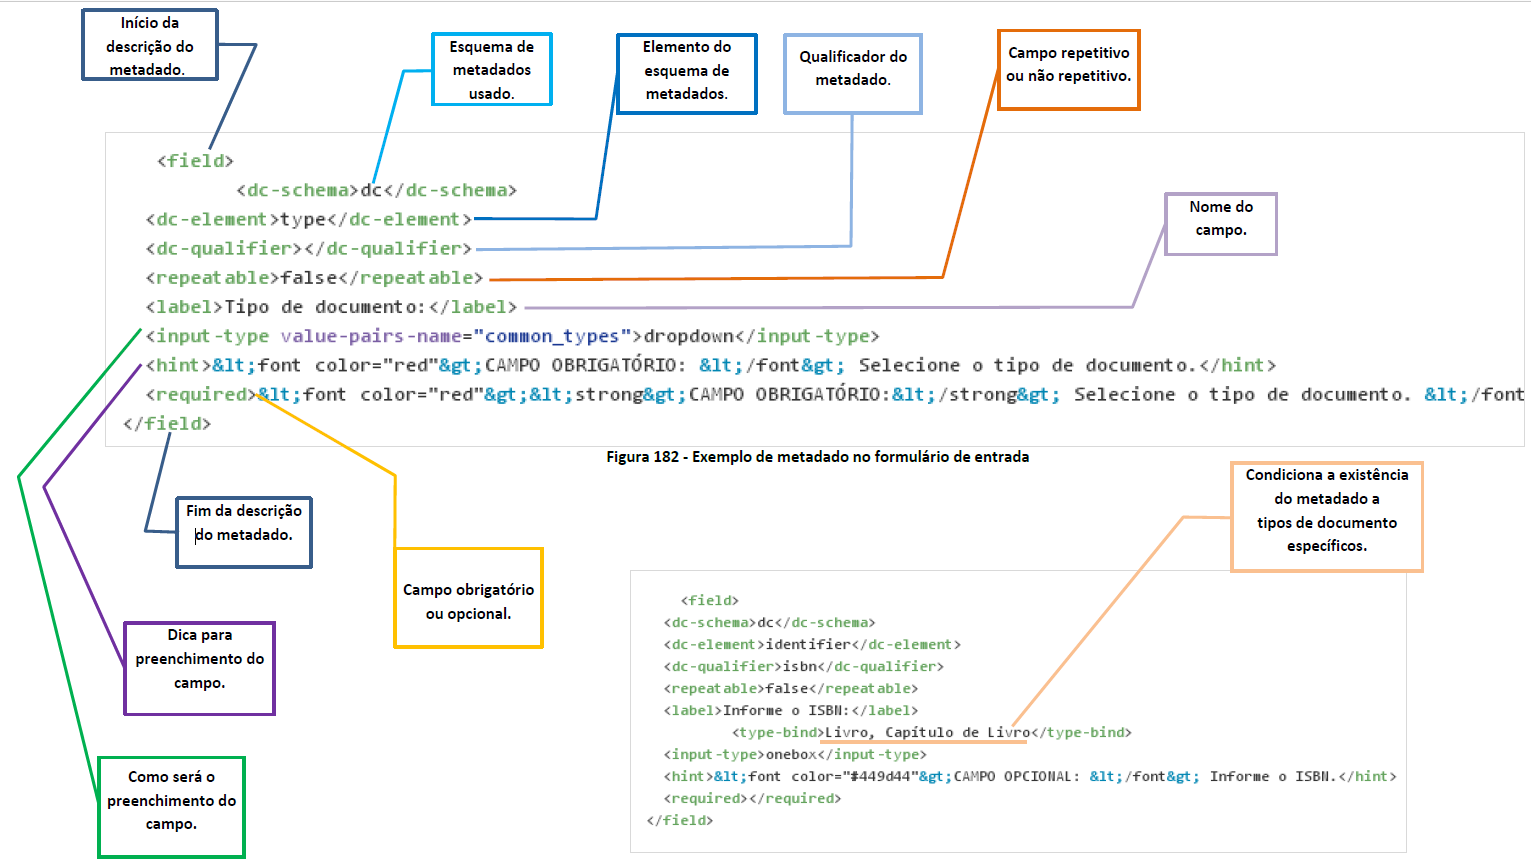
\includegraphics[scale=0.4]{figura/input-forms.png}
                \caption{Formulário de entrada}
            \label{Rotulo}
          \end{figure}
\newpage
    \subsection{Registrar metadados}
Para registrar novos metadados no DSpace é necessário inseri-los tanto via interface, o que será mostrado abaixo, quanto no formulário de entrada. Por padrão o DSpace utiliza uma versão qualificada do esquema Dublin Core. É possível também configurar outros esquemas de metadados no registro.
\singlespacing
Passo 1: Para registrar novos metadados ou alterar vá no menu do Administrador e em “Configurações gerais” e clique na opção <Registrar metadados>.
    
        \begin{figure}[!htp]
                \centering
                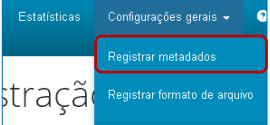
\includegraphics[scale=0.9]{figura/registrar-metadados-passo1.png}
                \caption{Registrar-metadados-passo-1}
            \label{Rotulo}
        \end{figure}

Passo 2: A página seguinte apresenta a lista dos esquemas registrados. Como será adicionado um metadado no Dublin Core (dc), clique no primeiro link como mostrado na figura abaixo.

         \begin{figure}[!htp]
                \centering
                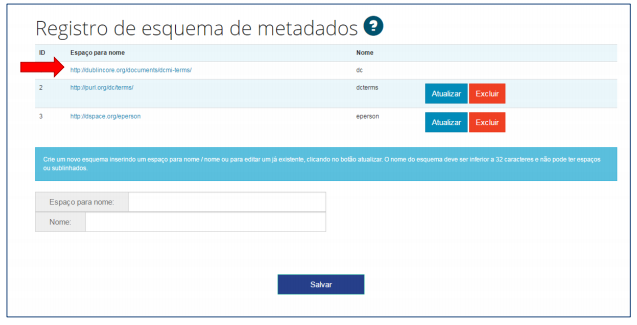
\includegraphics[scale=0.9]{figura/registrar-metadados-passo2.png}
                \caption{Registrar-metadados-passo-2}
            \label{Rotulo}
        \end{figure}
\newpage
Passo 3: Na página seguinte é fornecida uma lista dos metadados registrados, separando elementos e qualificadores e os comentários. É possível atualizar ou excluir esses metadados, clicando respectivamente em “Atualizar” ou “Excluir”. Para adicionar novo metadado, vá até o fim da página
        \begin{figure}[!htp]
                \centering
                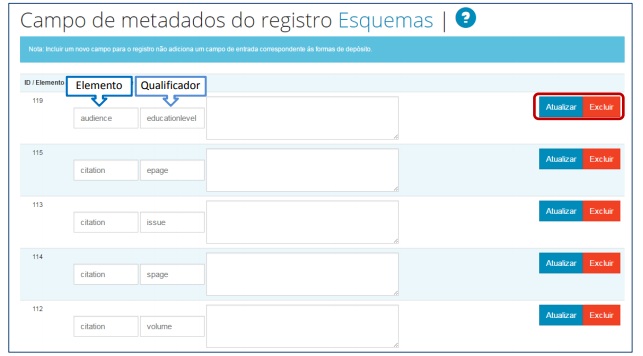
\includegraphics[scale=0.9]{figura/registrar-metadados-passo3.png}
                \caption{Registrar-metadados-passo-3}
            \label{Rotulo}
        \end{figure}

Passo 4: Em “Adicionar campo de metadado”, preencha os campos “Elemento”, “Qualificador” e “Nota de Escopo”. O preenchimento do qualificador e da nota de escopo não é obrigatório e pode ser deixado em branco. O qualificador quando preenchido NÃO pode conter espaços ou sublinhados. Depois de preenchido, clique em “Adicionar novo” e o metadado será criado.

        \begin{figure}[!htp]
                \centering
                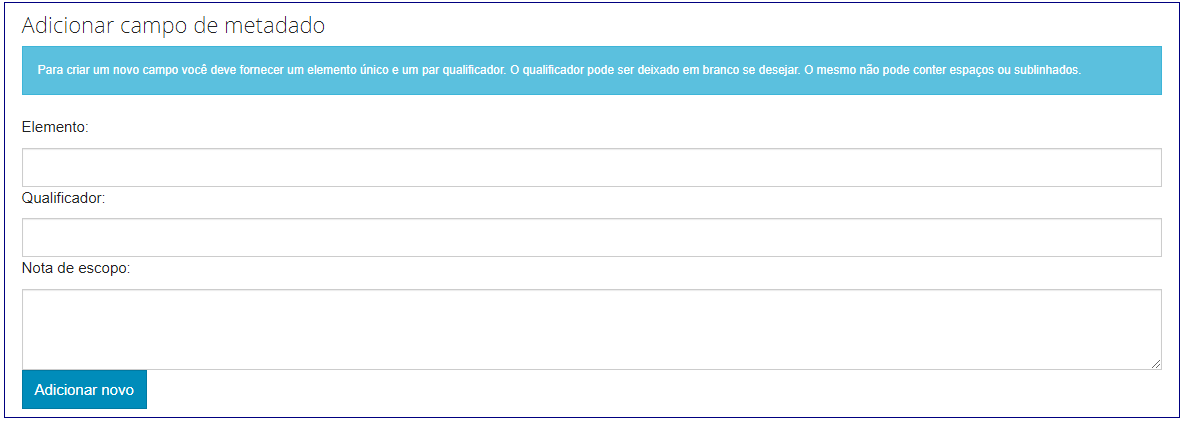
\includegraphics[scale=0.5]{figura/registrar-metadados-passo4.png}
                \caption{Registrar-metadados-passo-4}
            \label{Rotulo}
        \end{figure}

\newpage


\section{Upgrade de versões}
\newpage
\subsection{Upgrade de versões}
Realizar upgrade de versões não é uma tarefa simples e direta. Há alguns dificultadores, os mais comuns são:\\

\textbullet \hspace{6pt} Migrar as configurações antigas para a nova versão;\\
\textbullet \hspace{6pt} Migrar arquivos de layout que foram alterados pelo usuário;\\
\textbullet \hspace{6pt} Migrar as estatísticas antigas do solr;\\
\textbullet \hspace{6pt} Atualizar a base de dados;\\
\textbullet \hspace{6pt} Migrar a assetstore (pasta que contém os documentos);
\singlespacing
É possível perceber uma diferença entre os procedimentos descritos no manual oficial do DSpace 6.x e o que aqui se apresenta. De fato, entende-se que existe maior segurança em se realizar uma instalação clean da nova versão e se aplicar nela as configurações particulares da antiga. Essa tarefa gera também uma melhor compreensão do processo de atualização, e é possível estabelecer um procedimento genérico de migração de uma versão 1.x ou 3.x para a 6.x.
\singlespacing
Para melhor entender como é feita a atualização de versões, a figura abaixo descreve, de forma simples, os passos explicados nessa página:

\subsection{Backup}
Para o backup da base de dados basta que se execute o comando:

\begin{minted}{bash}
pg_dump dspace4x > bkp_dspace4x_DDMMAA.sql
\end{minted}

Já para o backup da(s) pasta(s) assetstore, basta que se execute o comando, para cada pasta utilizada (em geral só se utiliza uma única pasta, que deve estar dentro da pasta base de instalação. Contudo para se ter certeza de qual(is) pasta(s) é(são) utiliza(s), deve-se verificar no arquivo \textbf{dspace-4.x-base/config/dspace.cfg} os parâmetros \textbf{assetstore.dir, assetstore.dir.1 e assetstore.dir.2}, estando dentro da pasta dspace-4.x-base:   

\begin{minted}{bash}
tar -cvzf bkp_assetstore_DDMMAA.tar.gz assetstore
\end{minted}

O backup das estatísticas pode ser feito, dentro da pasta dspace-4.x-base/solr/, com:

\begin{minted}{bash}
tar -cvzf bkp_solr_DDMMAA.tar.gz data
\end{minted}

\subsection{Restore}

\textbf{Base de dados}
\singlespacing

A atualização do DSpace precisa da criação de um banco de dados novo, não é aconselhado utilizar o banco da versão anterior. Dessa forma, é necessário criar um novo banco de dados, \textbf{dspace6x}(nome ilustrativo)

%\textbullet \hspace{6pt} Remova e crie novamente a base de dados da nova instalação. Isso fornecerá uma base de dados vazia:

%\begin{minted}{bash}
%dropdb dspace6x
%\end{minted}


\begin{minted}{bash}

createdb --username=postgres --owner=dspace --encoding=UNICODE dspace6x

psql --username=postgres dspace6x -c "CREATE EXTENSION pgcrypto;"
\end{minted}

Acesse a pasta com o backup do banco de dados, \textbf{bkp $\_$ dspace4x $\_$ DDMMAA.sql}, e execute o comando de restauração para o bando \textbf{dspace6x}.

\begin{minted}{bash}
psql -d dspace6x -f bkp_dspace4x_DDMMAA.sql
\end{minted}

Finalizado a restauração do banco, acesse a pasta de binários do DSpace 6.3,
\begin{minted}{bash}
cd /dspace-base/bin
\end{minted}
e execute o comando,
\begin{minted}{bash}
./dspace database migrate
\end{minted}

\newpage
\subsection{Arquivos do repositório Assetstore}

O backup do arquivo dos repositório devem ser movidos para a pasta base do DSpace 6.3.
\begin{minted}{bash}
cp bkp_assetstore_DDMMAA.tar.gz /dspace-base/
\end{minted}
Em seguinda descompacte o backup,
\begin{minted}{bash}
tar -vzxf bkp_assetstore_DDMMAA.tar.gz
\end{minted}
renomei a pasta descompactada para assetstore
\begin{minted}{bash}
mv -R bkp_assetstore_DDMMAA assetstore 
\end{minted}


\subsection{Estatísticas}

O backup da estatística do Solr
\textbullet \hspace{6pt} Mova o arquivo backup da(s) assetstore(s) para dentro da pasta \textbf{dspace-6.x-base}, e lá execute o comando:

\begin{minted}{bash}
tar -vzxf bkp_solr_DDMMAA.tar.gz
\end{minted}

\subsection{Atualizar Sincronizar}

O DSpace, depois de adicionado as pastas de backup, deve ser atualizado a instalação do respositório. Acesse a pasta de instalação do DSpace,
\begin{minted}{bash}
cd /home/dspace/repositorio-padrao-dspace-6/target/dspace-installer/
\end{minted}
em seguida execute o comando do Ant, agora com comando de update.
\begin{minted}{bash}
/home/dspace/apache-ant…/bin/ant update
\end{minted}

Para atualizar os índices execute, dentro da pasta dspace-6.x-base/bin, os comandos:
\begin{minted}{bash}
./dspace index-discovery -f
\end{minted}

\newpage
\section{Layout}
\newpage

\subsection{home.jsp}

Uma parte crítica de qualquer atualização são as mudanças de layout. É necessário ter conhecimento de quais arquivos foram alterados, e sobrescrevê-los na interface de usuário jspui. 

Para fazer as alterações na página principal o arquivo para tal finalidade é o home.jsp

        \begin{figure}[!htp]
                \centering
                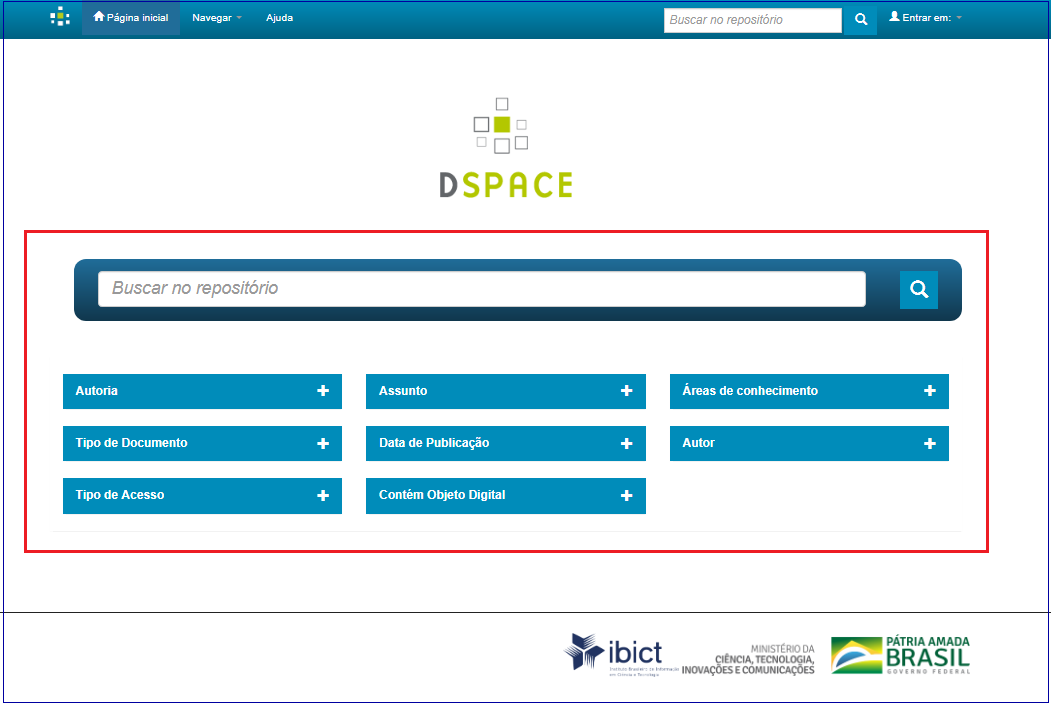
\includegraphics[scale=0.5]{figura/home.png}
                \caption{home.jsp}
            \label{Rotulo}
        \end{figure}

\subsection{navbar-default.jsp}
Para as alterações na página que se encontra no topo você deve se atentar para o navbar-default.jsp.

\begin{figure}[!htp]
                \centering
                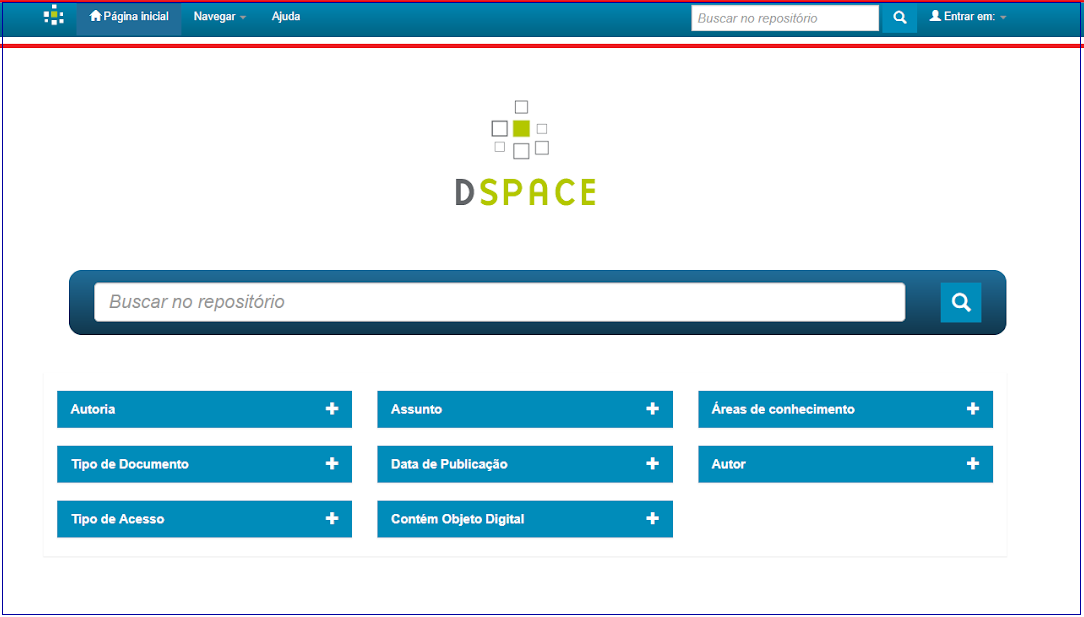
\includegraphics[scale=0.5]{figura/navbar-default.png}
                \caption{navbar-default.jsp}
            \label{Rotulo}
        \end{figure}

\newpage  

\subsection{Webui-browse-index}

Para a inclusão dos metadados na barra do “navegar”. 

    \begin{figure}[!htp]
        \centering
        \includegraphics[scale=0.5]{figura/navegar1.png}
        \caption{navbar-default.jsp}
        \label{Rotulo}
     \end{figure}



É feita no arquivo dspace.cfg, localizado em /dspace-base/config/ e são incluídas nas variáveis webui.browse.index


    \begin{figure}[!htp]
        \centering
        \includegraphics[scale=0.5]{figura/webui-browse-index.png}
        \caption{navbar-default.jsp}
        \label{Rotulo}
    \end{figure}
 
\newpage
\subsection{Inclusão das imagens}
       
Para a inclusão da imagem que se encontra no topo.

\begin{figure}[!htp]
        \centering
        \includegraphics[scale=0.5]{figura/logo-topo.png}
        \caption{navbar-default.jsp}
        \label{Rotulo}
    \end{figure}
    
A imagem tem que ser adicionada em \textbf{/home/dspace/apache-tomcat/jspui/image/}  
\singlespacing
Assim como, tem que ser informado o caminho da imagem nos arquivos navbar-admin.jsp e navbar-default.jsp, que ficam localizadas em: \textbf{/home/dspace/apache-tomcat-x.x.x/webapps/jspui/layout/}  

\begin{figure}[!htp]
        \centering
        \includegraphics[scale=0.3]{figura/dspace-logo-only1.png}
        \label{Rotulo}
    \end{figure}
    
\begin{figure}[!htp]
        \centering
        \includegraphics[scale=0.3]{figura/dspace-logo-only2.png}
        \caption{navbar-admin.jsp e navbar-default.jsp}
        \label{Rotulo}
    \end{figure}

Em relação a inclusão da logo principal.
\begin{figure}[!htp]
        \centering
        \includegraphics[scale=0.5]{figura/logo-principal.png}
        \caption{}
        \label{Rotulo}
    \end{figure}
    
\newpage 
A imagem tem que ser adicionada em \textbf{/home/dspace/apache-tomcat/jspui/image/} 
Assim como, tem que ser informado o caminho da imagem no arquivo header-default.jsp, que fica localizado em:  \textbf{/home/dspace/apache-tomcat-x.x.x/webapps/jspui/layout/}
    \begin{figure}[!htp]
        \centering
        \includegraphics[scale=0.5]{figura/footer-default.png}
        \caption{footer-default.jsp}
        \label{Rotulo}
    \end{figure}
    
\end{document}